\label{chap:2}
% Basics about PUFs in cryptography. How a key generator and a TRNG are used, encryption and decryption processes described 4-5 Páginas

This chapter presents an introduction to the concept of Physical Unclonable Functions (PUFs). After a brief description of their main characteristics and applications, the most common implementations are reviewed. The metrics selected to evaluate PUFs are then defined and the HDAs used to enhance their performances are introduced. 

\section{What is a PUF?}
The term Physical Unclonable Function (PUF) was coined by Tuyls et al. in \cite{Tuyls2007} and has become the prevalent term, but the notion of ``Physical one way function'' was first introduced by Pappu in \cite{Pappu2002}. There are multiple definitions given for PUFs \cite{Xu2015,Bohm2013}, but, in general, it is an entity that takes advantage of process variations on a measurable physical property to generate an unpredictable and unique response to a device. Process variations are the naturally occurring disparities between components with identical design during manufacture. This disparity is small and can not be modelled or replicated even by the designer or the manufacturer of the device. 


PUFs can be thought of as a black-box challenge-response system \cite{Herder2014}. If a challenge $c$ is issued, it returns a response $r=f(c)$. This forms a challenge-response pair (CRP). The fundamental aspect of PUFs is that $f$ (Input/output relations in the PUF) is hidden from the user or the potential attacker.

The essential characteristics that must be present in a PUF's response are \textbf{uniqueness} (how unique is the response of a particular instance among a group of instances of the same type),  \textbf{unpredictability} (how unpredictable the response is even with knowledge of part of the response or of another PUF's response) and \textbf{reliability}  (how reproducible the PUF response is when the same challenge is applied at different points in time). Considering three PUFs named A, B and C and their corresponding CRPs, these PUFs characteristics are schematically depicted in fig. \ref{fig:req}.

\begin{figure}[H]
    \centering
    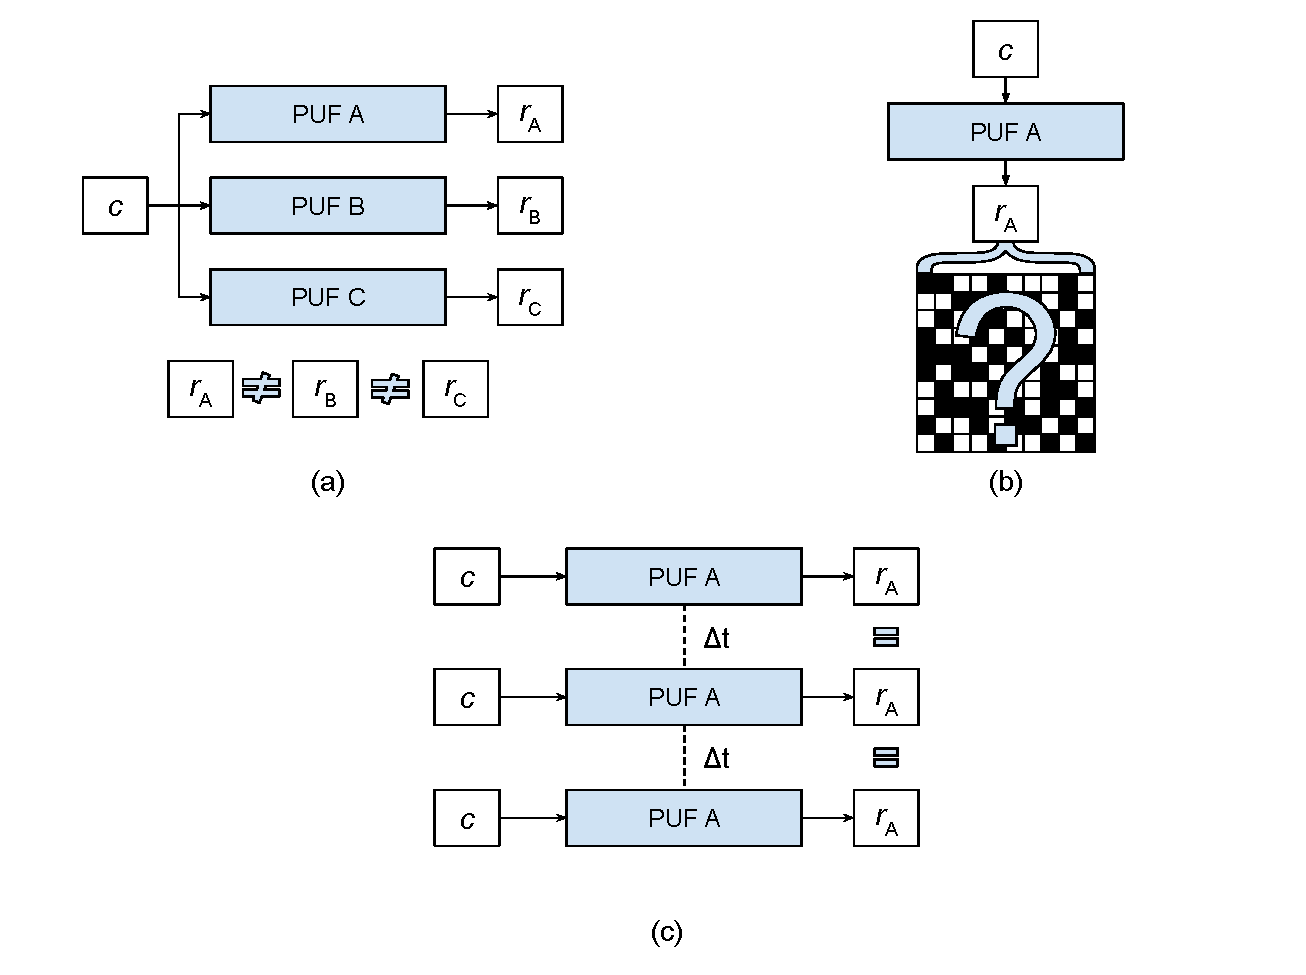
\includegraphics[width=15cm]{images/PUF requirements.pdf}
    \caption{Desired characteristics in a PUF's response: (a) represents uniqueness, (b) unpredictability and (c) reliability. }
    \label{fig:req}
\end{figure}

PUFs can be distinguished between weak or strong according to the amount of CRPs available \cite{Herder2014}. A weak PUF will support a small amount of challenges. Therefore, the CRPs must be kept secret, otherwise the PUF can be emulated. In some cases there may be only one challenge and accordingly only one CRP. Strong PUFs on the other hand have such a large amount of CRPs that they cannot be mapped in a reasonable time frame. Due to this, its output does not need to be private. It should not, however, reveal information about the functionality of the PUF since, otherwise, responses to different challenges could be predicted. 




% Regarding actual implementations, many different approaches have been published since the concept of PUFs can be applied to plenty of physical phenomena. A  comprehensive list is found in \cite{Maes2010}. Some non-electric PUFs include the pioneer optical PUF \cite{Pappu2002} or paper PUFs \cite{paperpuf}. However, most PUFs are electrical since they are easier and less costly to implement in an electronic medium. They are based on manufacturing variations that cannot be controlled or predicted. Some of the better known ones are arbiter PUFs, ring oscillators and SRAM PUFs. 

% Arbiter PUFs \cite{Arbiter} introduce a digital race condition on two paths on a chip. An arbiter circuit decides which path is faster, resulting in two possible states.  A ring oscillator is a device composed of an odd number of inverters. In ring oscillator PUFs \cite{oscillatorog,Suh2007}, the differences in frequency of symmetric ring-oscillators are measured. Finally, SRAM PUFs use the difference in strength of the two inverter's of an SRAM cell which result in a certain power-up state (``1'' or ``0''). A more detailed look into SRAMs and their use as a PUF is done in chapter \ref{chap:3} since they are the focus of study in this work. 

\section{PUF applications}
\label{sec:applications}
PUFs have a variety of applications but almost all of them are geared towards security, particularly for digital devices \cite{Maes2010,Bohm2013,Xu2015}. They are used as one of the main components to build RoT or hardware anchors to reinforce security in the device in which the RoT is incorporated. The PUF response acts as the foundation to derive trust for the rest of components of the device. 

Several ways to design and develop a RoT are presented in literature. A rough classification can be provided according to the implementation nature. A RoT can be implemented in hardware, software or a hybrid hardware/software version. The main advantage of hardware RoT compared to software RoT is being invulnerable to malware attacks. One of the most popular technologies to implement hardware RoT is the Trusted Platform Module (TPM) \cite{TPM}. It is a standard for a secure cryptoprocessor, which is a dedicated microcontroller with the required security primitives to ensure the integrity of the device. This includes the generation and storage of cryptographic keys and true random number generation, and requires physical security mechanisms to provide anti-tamper protection. However, they involve a large cost in terms of area and power which is suitable for in small, resource constrained applications such as those of Internet of Things (IoT) or embedded devices.

PUFs offer two advantages in this field compared to the conventional hardware RoT solutions: cost reduction and an increased level of security. Regarding cost, secret information to derive cryptographic keys are stored in a secure NVM for traditional systems. Meanwhile, a PUF's response is used for generation of keys on-the-fly without being necessary their storage in NVMs. Furthermore, the PUF existing implementations are not expensive in terms of energy and area. Some PUF implementations even use already existing circuitry of the device, which further reduces these costs. Regarding security, PUFs are practically impossible to attack through reverse engineering methods due to their unclonability. As mentioned before, the response is generated on-chip. This is an advantage in terms of security as well, since the traditional method of transferring secure information to the chip is an additional vulnerability against eventual attacks. Furthermore, since PUFs rely on small process variations, they have an innate protection against physical tampering as any meddling may modify the response and turn the PUF unusable. 

In the next subsections different security applications of PUFs are presented.

\subsection{PUF as a unique identifier}

Since PUFs generate a unpredictable and unique response, they can be used directly for identification \cite{McGrath2019,Maes2010,,Okumura2011}. Each unique PUF is assigned to one physical system. In this way, PUF identification is similar to biometrical identification. The PUF output constitutes the ``digital fingerprint'' of the system.

A simple example of the use of a PUF as an unique identifier is shown in fig. \ref{fig:id}. Two phases can be distinguished when using a PUF as an unique identifier: enrollment and identification. During enrollment, shown in fig. \ref{fig:id} (a), a number of CRPs from every PUF are stored in a database coupled with the physical system associated with the PUF. This step is done only once. Later, during identification, shown in fig. \ref{fig:id} (b), the verifier selects one challenge from the database and challenges the PUF with it. If the resulting response matches the stored one, the identification is positive, and, otherwise, it fails.

In strong PUFs, where multiple CRPs are stored, there can be a degree of tolerance with the discrepancies between the responses \cite{Maes2010}. This is due to the fact that each CRP is used only once to prevent replay attacks. In weak PUFs, there is only a small number of possible challenges so the verification response should match perfectly the enrollment response. The PUF must be examined in an environment where an authenticating party is present to ensure that the PUF itself is being evaluated and there are no replay attacks. 

\begin{figure}[H]
    \centering
    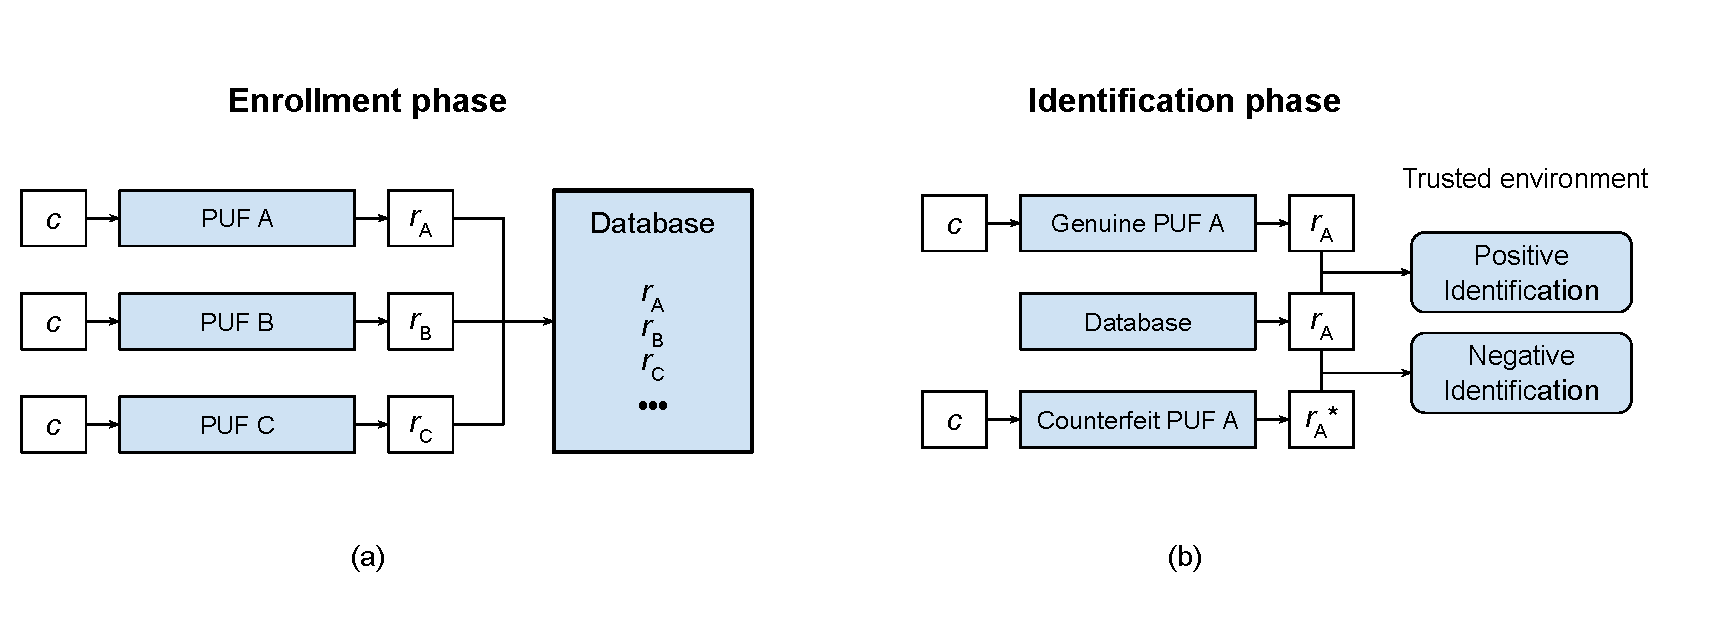
\includegraphics[width=15cm]{images/Weak ID.pdf}
    \caption{Simple implementation using a PUF as an unique identifier.  (a) Enrollment: occurs only once. (b) Identification: occurs any time the system has to be identified.}
    \label{fig:id}
\end{figure}

% System identification is important in multiple fields. They can be used for example to authenticate products in supply chains. Production of many goods involves shipping across multiple countries and controlling every step related to the product is becoming increasingly difficult. Accordingly, counterfeit or malicious components are a rising problem in today's supply chains. Malfunction or the malicious use of sensitive data can be disastrous in these cases. 

\subsection{PUF as a secret key generator}
\label{sec:enc/dec}
PUFs can be used as well for key generation in cryptographic encryption and decryption algorithms \cite{Suh2007,Rahman2016,Herder2014}. Traditionally, the key is permanently stored in a NVM, which opens up multiple points of attack. However, PUFs generate the key whenever required instead of storing it, providing better security. This application has strict requirements for the response as it must be perfectly reliable and unpredictable to ensure the security of the cryptographic scheme. Weak PUFs that provide only one response are optimal for secret key generation \cite{Maes2010}, as only one key is required in cryptographic algorithms.

An important distinction can be made between symmetric and asymmetric cryptographic algorithms. In symmetric key algorithms, shown in fig. \ref{fig:symm_crypt}, the same key is used for both encryption and decryption. This means that the key must stay secret during the whole process. The key has to be provided to the receiver in advance for authentication through a secure channel, which in some applications is complicated and opens up more points of attack \cite{Gao2020}.

\begin{figure}[t]
    \centering
    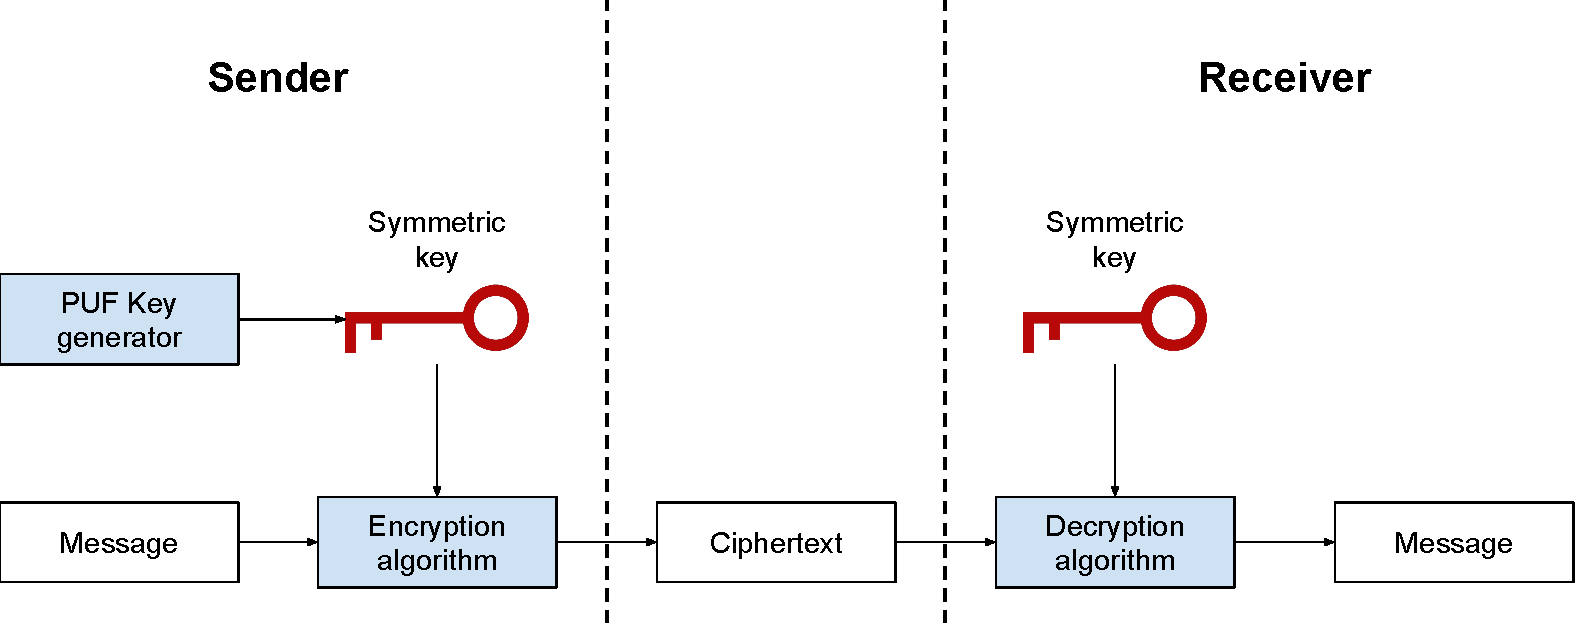
\includegraphics[width=14cm]{images/Symmetric key generation.pdf}
    \caption{Use of a PUF as a key generator in a symmetric cryptographic algorithm.}
    \label{fig:symm_crypt}
\end{figure}


On the other hand, asymmetric or public key algorithms use different keys for encryption and decryption. One of the keys can be public, knowing it will not compromise the security of the system. Having a public key algorithm instead of a symmetric one is useful when secure channels are not available, the number of participants in the encryption is high, or when keys are frequently changed but the security requirements are higher. 

In a public key algorithm, first the PUF device generates a key used to create a private and public key pair (fig. \ref{fig:asymm_crypt} (a)). The public key is broadcast on a public key server that any party can access. From here, there are different applications. The PUF device can be authenticated by sending certain data to be encrypted by the private key. If the original data is recovered through the public key, the PUF device is correctly verified. Similarly, any transaction signed by this private key can be verified through the public key. Device-to-device secure communication is another possibility, where a certain message encrypted by the sender through the public key can only be decrypted and read by the intended receiver through the private key (fig. \ref{fig:asymm_crypt} (b)).




\begin{figure}[H]
    \centering
    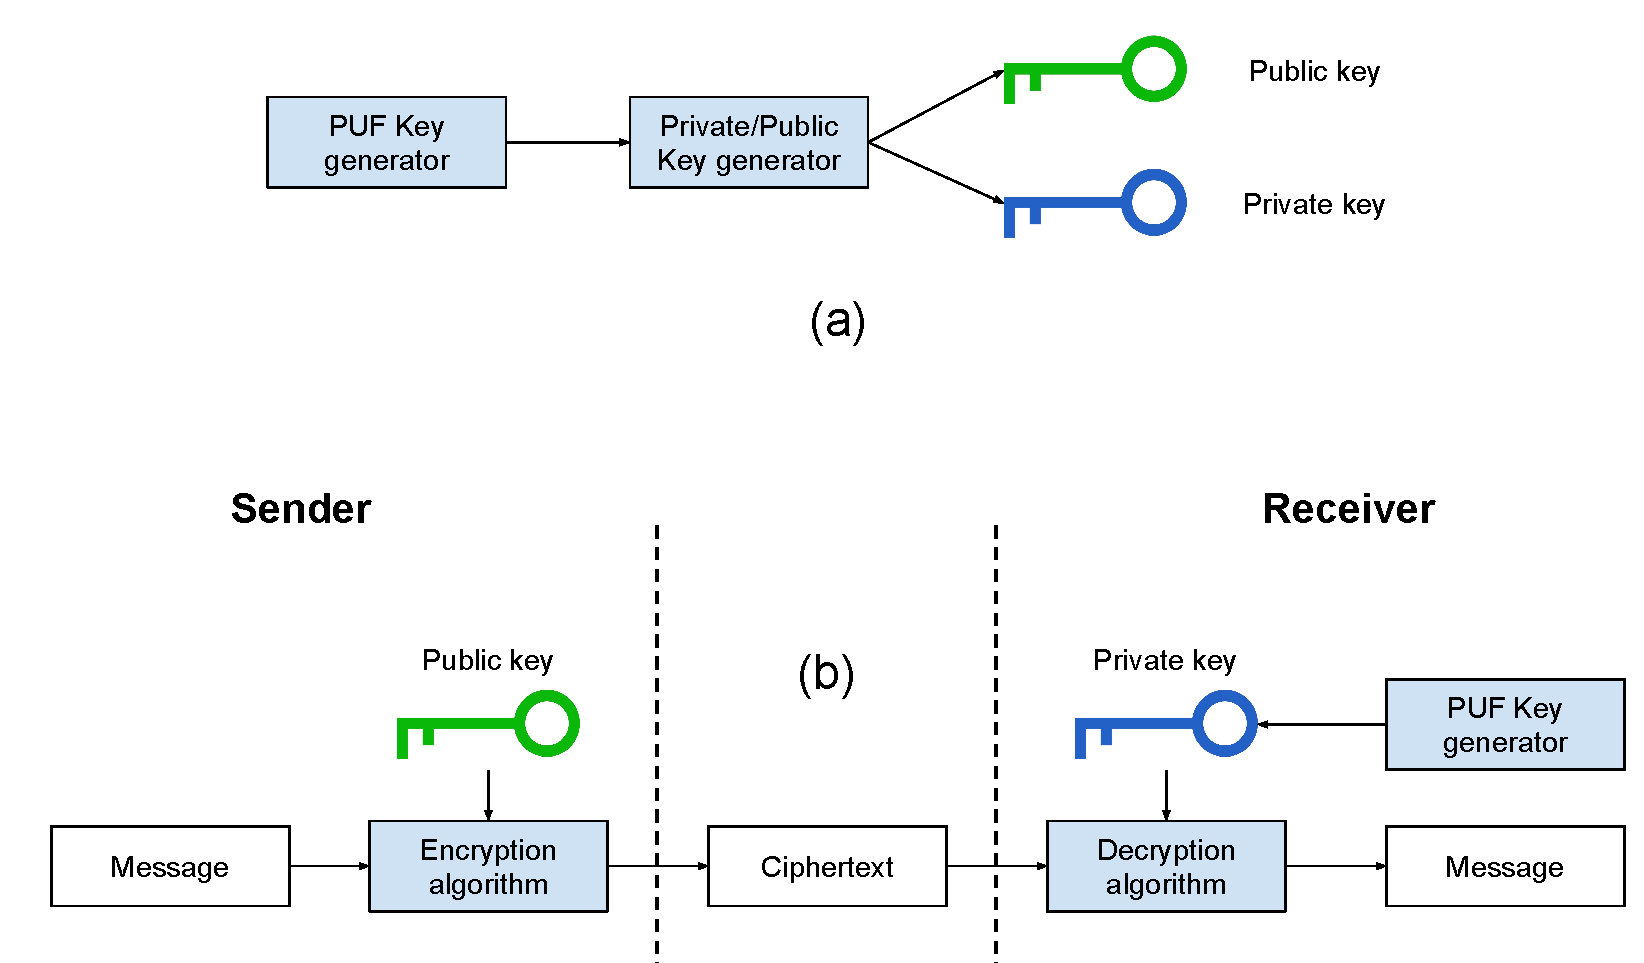
\includegraphics[width=14cm]{images/Asymmetric key generation.pdf}
    \caption{Use of a PUF as a key generator in a public key algorithm.}
    \label{fig:asymm_crypt}
\end{figure}


The requirements in terms of minimum key length for these algorithms can vary greatly, from 128 bits for the symmetric algorithm AES \cite{AES} to 2048 for the asymmetric RSA algorithm \cite{RSA}. The chosen algorithm and entailed level of security will require different lengths, but the bare minimum is 128 bits \cite{Alioto2019}.

% These algorithms are the foundation of digital security, used to establish secure communications channels, validate digital signatures or verify elements of an IoT network to name a few examples.  
%Generating the key consists in simply measuring the output of the PUF. This key will be used along with an encryption algorithm to encrypt a plain text and to decrypt the cipher. The strength of symmetric key algorithms are based on their resistance to brute force attacks, where all possible combinations are tried. The Data Encryption Standard (DES) developed in the early 1970s by IBM was the standard for encryption algorithms, but its short length (56 bits) made it susceptible to attacks as computing power kept growing \cite{Stallings}. The advanced encryption standard (AES) \cite{Daemen} was instead adopted in the early 2000s and has since become the new standard, since it allows for keys of 128, 192 and 256 bits. These lengths are invulnerable to a brute force attack in a practical sense, since $2^{128}$ or $2^{256}$ combinations are both very large numbers. 

% The security provided by keys of either length is effectively identical with conventional technology, but not with quantum computing in mind. A quantum computer can complete a brute-force attack on a key of length $n$ in the time it would take the traditional computer to find a key of length $2n$ \cite{bennett1997strengths}. Accordingly, a key of length 128 is reduced to the security of a key of 64, which is breakable in a reasonable time frame. Even though quantum computers are far from reaching the capabilities of today's traditional computers, there are cases where security is more important than the cost of generating a key of 256 bits or the cost itself is very low. 256 bit keys are adopted so that the system is future-proof and safe against the possibility of great advances in quantum computing in a short time.


% On the other hand, asymmetric or public key algorithms use different keys for encryption and decryption. One of the keys can be public, knowing it will not compromise the security of the system. Having a public key algorithm instead of a symmetric one is useful when secure channels are not available, the number of participants in the encryption is high, or when keys are frequently changed. Accordingly asymmetric encryption is mostly used in day-to-day communication channels, especially over the Internet. They are used as well in IoT networks and for digital signatures, to name a few examples. These technologies are already ubiquitous and keep growing, so public key algorithms are of great importance.

% They come however at a higher computational cost \cite{salomaa2013public}. Public keys can also suffer from man-in-the-middle attacks. In these, the transmission of public keys is intercepted and then modified to provide different public keys to the receiver. This allows the attacker to read the private data while avoiding suspicion. The main systems where this attack is dangerous is where the communications hardware is controlled by the adversary, such as in the Internet or public networks. They are vulnerable to related key and brute-force attacks as symmetric key algorithms. However, brute-force attacks are more effective against asymmetric key algorithms. These algorithms, such as RSA (based on prime factorization) or elliptic curve cryptography (based on the algebraic structure of elliptic curves over finite fields) are based on the difficulty to solve certain mathematical problems. While these are very difficult to solve in terms of processing, they are not as difficult as trying all possible combinations. This results in an effective security lower than the key length. For example, 2048-bit RSA keys are the minimum recommended and they are equivalent to 112-bit symmetric keys. On top of that, these algorithms are turn completely obsolete by quantum computer due to the use of Shor's algorithm \cite{chen2016report}

% Hybrid systems exist as well, where an asymmetric key algorithm is used to verify a secure channel. Once the channel is verified symmetric key algorithms are employed due to their reduced computational cost. 

\subsection{PUF as a source of entropy}
\label{ss:entropy}
True random number generators (TRNG) generate random numbers from unpredictable physical processes. Although their main field of application is in cryptography, they are used in gambling as well as in situations were randomness is useful, such as juror selection or military draft lotteries. One example of their use in cryptography is to generate nonces \cite{Alioto2019}, an arbitrary number employed just once in a cryptographic communication to avoid replay attacks \cite{Martinez-Rodriguez2018}. These nonces can be used as initialization vectors (IVs) to prevent a sequence of text that is identical to a previous sequence from producing the same exact encrypted message. PUFs that can perform both as a key generator and as a source of entropy are specially useful in cryptographic algorithms \cite{Holcomb2009,Baturone2015}. 

PUFs used as a source of entropy take advantage of the unpredictability of PUF implementations (fig. \ref{fig:dice}). In terms of reliability they ideally require the exact opposite of the applications presented so far: a completely random response. To quantify the entropy or randomness of a PUF response, NIST tests \cite{Rukhin2010}, developed by the National Institute of Standards and Technology, can be used. 

\vspace{0.5cm}

\begin{figure}[H]
    \centering
    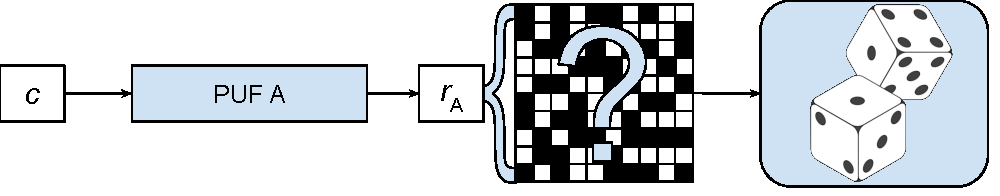
\includegraphics[width=15cm]{images/RNG.pdf}
    \caption{Use of a PUF as a source of entropy.}
    \label{fig:dice}
\end{figure}



\section{PUF Implementations}
\label{sec:implementations}
%Different types of PUF implementation, arbiter, ring oscillator bi-stable PUFS. 3-4 Páginas


In this section a brief overview of different PUF implementations is provided. Many different approaches have been published, since the concept of PUFs can be applied to plenty of physical phenomena. Some implementations take advantage of already existing properties of the system they secure, while others are embedded. The implementations presented here cannot be taken as a complete list, only some of the most significant ones are considered. A more comprehensive listing can be found in \cite{McGrath2019,Maes2010}. 

\subsection{Optical and non-electric PUFs}

 The original optical PUF presented in \cite{Pappu2002} relies on the interaction of a laser beam with a scattering medium in its path. As shown in fig. \ref{fig:opticalpuf}, the input is the position and polarization of the laser (strong PUF) and the output is the "speckle" of light exiting the scattering medium, which is recorded by an imaging device. A hash is applied to this recording to obtain a string of bits. The scattering path depends heavily on the input and the structure of the scattering medium, and unless this medium is very simple it is practically impossible to model and predict the output. In the mentioned implementation, microscopic refractive glass spheres embedded in a transparent epoxy plate are used as scattering medium. This implementation is not practical due to the complexity of the system, it served as a proof of concept. A more integrated design was proposed in \cite{Tuylsoptic} and more recently in \cite{Rhrmair2013OpticalPR}. Optical PUFs provide an unmatched input/output complexity which cannot be obtained by electrical PUFs, but their high cost make them hard to justify in real implementations. 
 
 \begin{figure}[H]
    \centering
    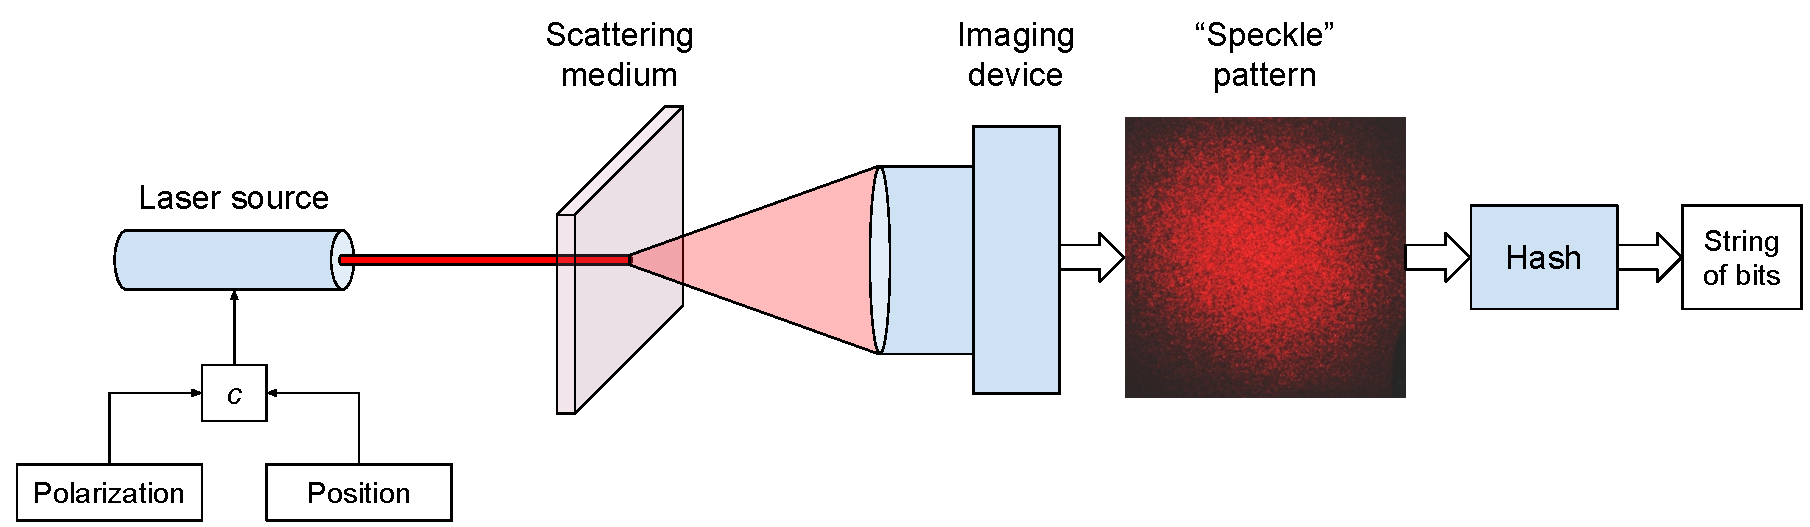
\includegraphics[width=15cm]{images/Optical PUF.pdf}
    \caption{Schematic illustration of an optical PUF implementation.}
    \label{fig:opticalpuf}
\end{figure}

Electrical or silicon-based PUFs are naturally easier to implement in an electronic medium and less costly, so the rest of the designs considered are electrical. There are, however, other proposed non-electrical PUFs such as Paper PUFs (using the unique fiber structure mainly for currency notes) \cite{paperpuf}, CD PUFs (using the lands and pits on a compact disk for identification) \cite{Hammouri2009CDsHF} or Acoustical PUFs (using the characteristic frequency spectrum of an acoustical delay line) \cite{mastersthesis}. The difference between these goes to show how versatile and universal the concept of PUF is, and more possible implementations come up as time goes by \cite{McGrath2019}. 

\subsection{Arbiter PUFs}

The initial proposal for an arbiter PUF was made in \cite{Arbiter}. It is considered a delay PUF. This type of PUFs exploit the random variations in delays of wires and gates on silicon. Arbiter PUFs introduce a digital race condition on two paths on a chip. An arbiter circuit decides which path is faster. They are designed in an identical way so that the resulting difference in delay is a product of manufacturing variations which cannot be controlled. The initial design uses \textit{switch} blocks connected in series with two states, where each state uses a different connection (\textit{straigh} or \textit{switched}). The challenge of the PUF will be the setting of the switches. In this way, the number of CRPs depends exponentially on the number of switch blocks used and it constitutes a strong PUF. Fig. \ref{fig:arbiter} shows a schematic for an arbiter PUF. 


\begin{figure}[H]
    \centering
    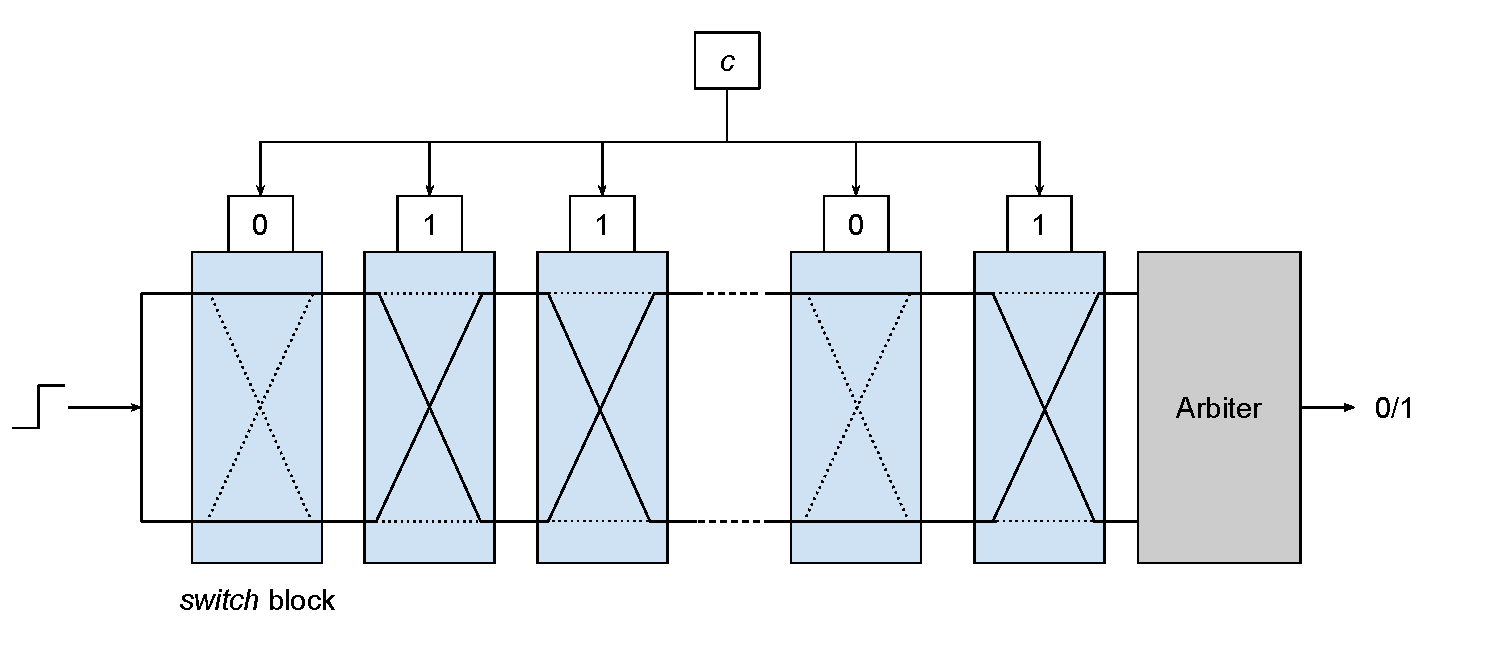
\includegraphics[width=15cm]{images/Arbiter.pdf}
    \caption{Schematic of an arbiter PUF implementation.}
    \label{fig:arbiter}
\end{figure}


These responses can however be noisy. If the offset between the two paths is too small, the setup-hold time of the arbiter is violated and the result will depend on random noise, causing unreliable bits. Environmental factors such as temperature, supply voltage or aging play a significant role in which path is faster as well.
Delays in each switch are linear and independent from each other, so arbiter PUFs with this design are vulnerable to the use of standard linear system analysis to model them and predict their response \cite{Arbitermaster}. To solve this, non-linearities are introduced. These come at the cost of even more noisy results and even if the response is less predictable it can still be modelled \cite{Maes2010}.

\subsection{Ring oscillator PUFs}

 A Ring Oscillator (RO) is a device composed of an odd number of inverters attached in a chain where the output of the last inverter is fed into the first one. Accordingly, the output oscillates between high and low voltage. Its oscillation frequency ($\nu$) depends on the sum of the gate delays of all inverters, and their structure is very simple (composed only of standard logic gates), so it can be easily implemented in a field-programmable gate array (FPGA) or an application-specific integrated circuit (ASIC). 

The RO PUF, first proposed by Gassend et al. in \cite{oscillatorog}, measures the difference in oscillation frequencies between pairs of identically designed ROs caused by manufacturing variations. Like arbiter PUFs, they fall under the delay PUFs category. Figure \ref{fig:ring oscillator} illustrates a standard RO-PUF implementation. It includes $N$ identically laid out ROs, two $N$-bit multiplexers, two counters and a comparator. Since the delay of each inverter will be different due to process variability, the frequency of each RO will be unique. The outputs of these ROs are fed into the multiplexers, and the PUF challenge determines which ROs are compared. The frequency is measured through the counters, which count the number of oscillations for a fixed interval of time. Finally, the output bit is determined based on which oscillator has a higher frequency, i.e. has a greater count.

\begin{figure}[H]
    \centering
    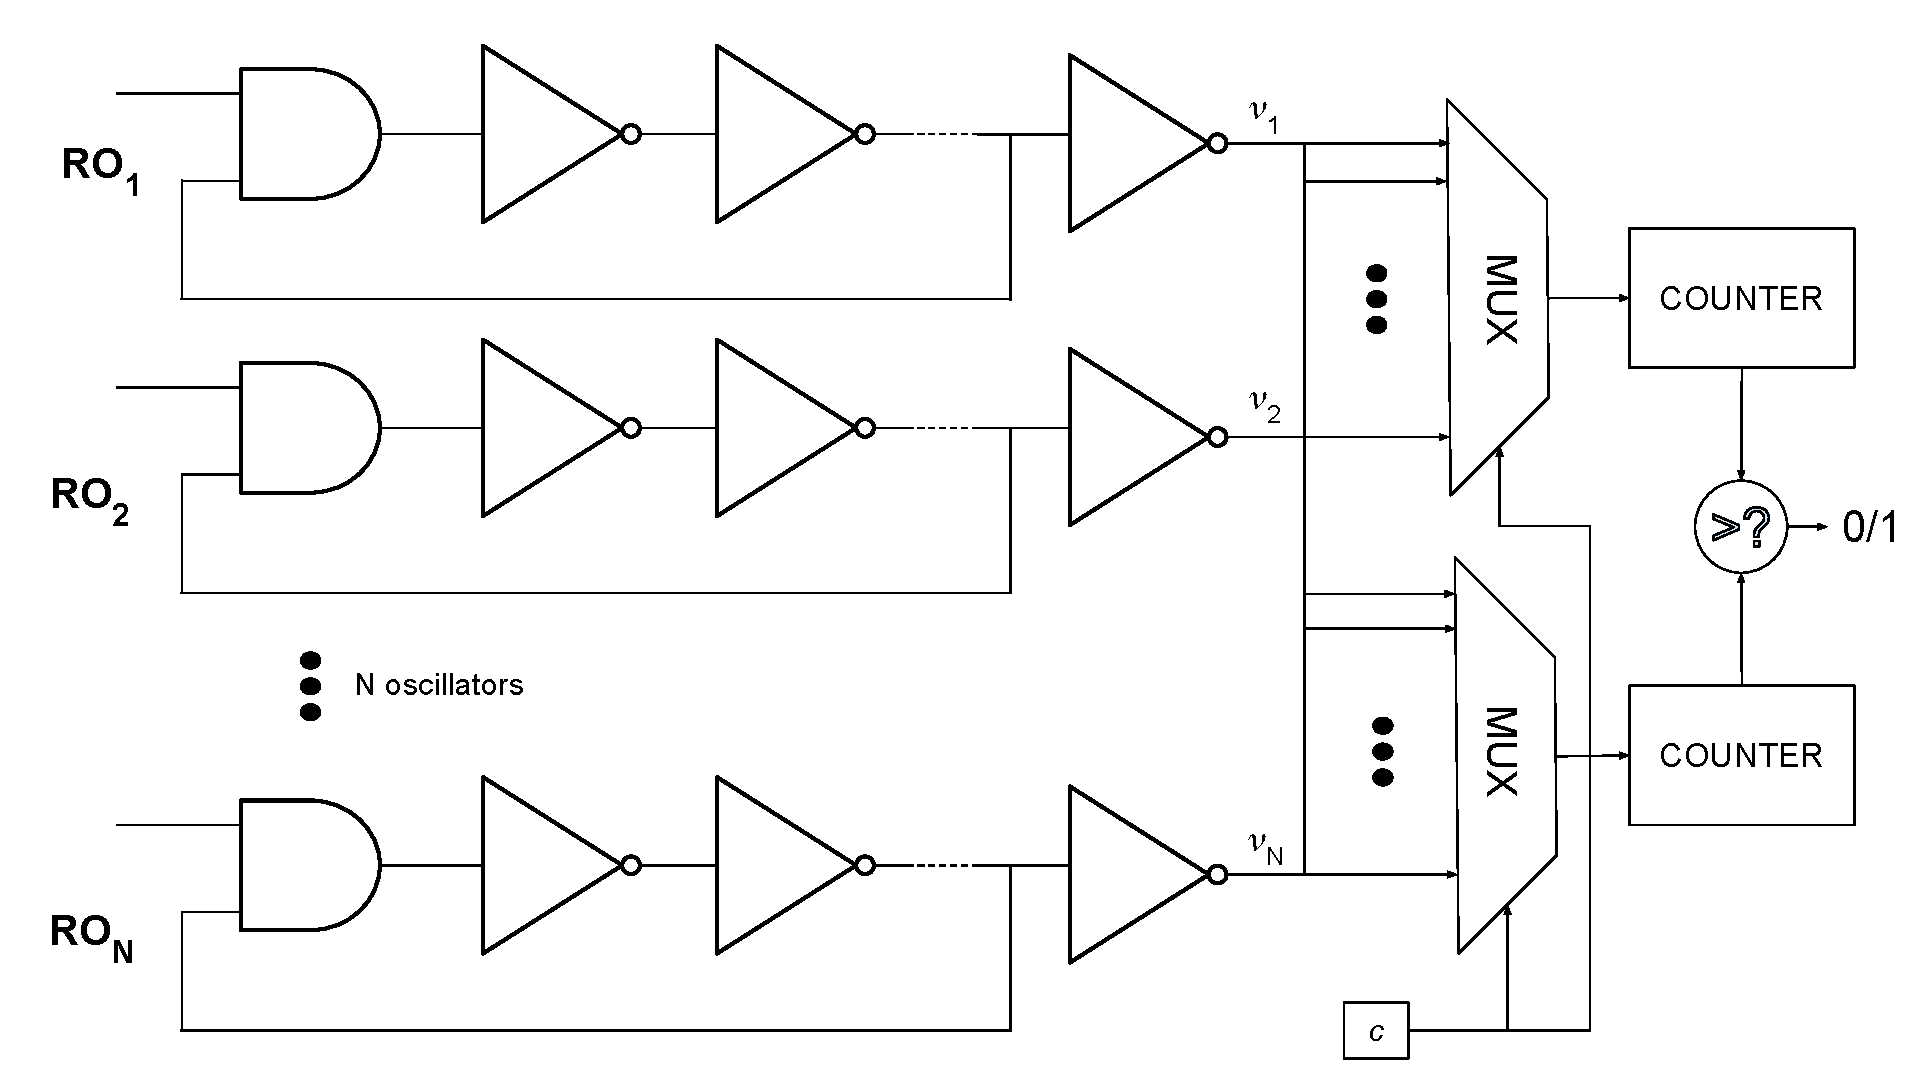
\includegraphics[width=14cm]{images/Ring oscillator.pdf}
    \caption{Schematic of a conventional RO PUF implementation.}
    \label{fig:ring oscillator}
\end{figure}

For $N$ oscillators, up to $log(N!)$ bits can be extracted by comparing frequencies. More pairings are possible but they would start to correlate with each other, compromising the security. This is a weak PUF, as there is a limited number of bits that can configure the PUF's operation. As in the case of the arbiter PUFs, RO PUFs are very susceptible to environmental variations since they are based on delay, and responses can be noisy. 




% \subsection{Coating PUFs}

% Coating PUFs were introduced in \cite{coating}. They use the protective coating that covers an integrated circuit (IC). The coating is doped with dielectric particles. In this way, they rely on both the randomness of manufacturing and the size, shape and location of the particles. An array of sensors measure the capacitance of the coating, and this capacitance is used to characterize the IC.  These PUFs provide good experimental results in terms of randomness and noise \cite{coating}. Their main drawback is the need for a specific manufacturing process. The other electric PUFs use simpler and easier to implement designs.

\subsection{SRAM PUFs}
\label{ss:cap2SRAM}
The first SRAM PUF was proposed separately by Guajardo and Holcomb in 2007 \cite{Guajarado_og,Holcomb2007InitialSS}. They use the start-up value of SRAM cells, which consist of cross-coupled inverters and are used as static memory. Before the cell powers up, the SRAM does not have any value stored since it is a volatile memory. Once it powers up, it theoretically exists in a metastable state where the two inverters are identical. However, due to mismatch from process variation, one of the inverters starts conducting before the other. Due to the positive feedback present in the cross-coupled inverters the cells settles in either ``1'' or ``0'' depending on which inverter powers up faster, as shown in \ref{fig:SRAM_PUF}. This state is used as the response. Whether one loop or the other is stronger depends on the relative threshold voltage between the transistors. This behaviour can be exploited to obtain a PUF. A response can be generated by using a number of cells, one per each desired bit. This is an extreme example of a weak PUF , since there is only one challenge (powering up) and one response. 

\begin{figure}[H]
    \centering
    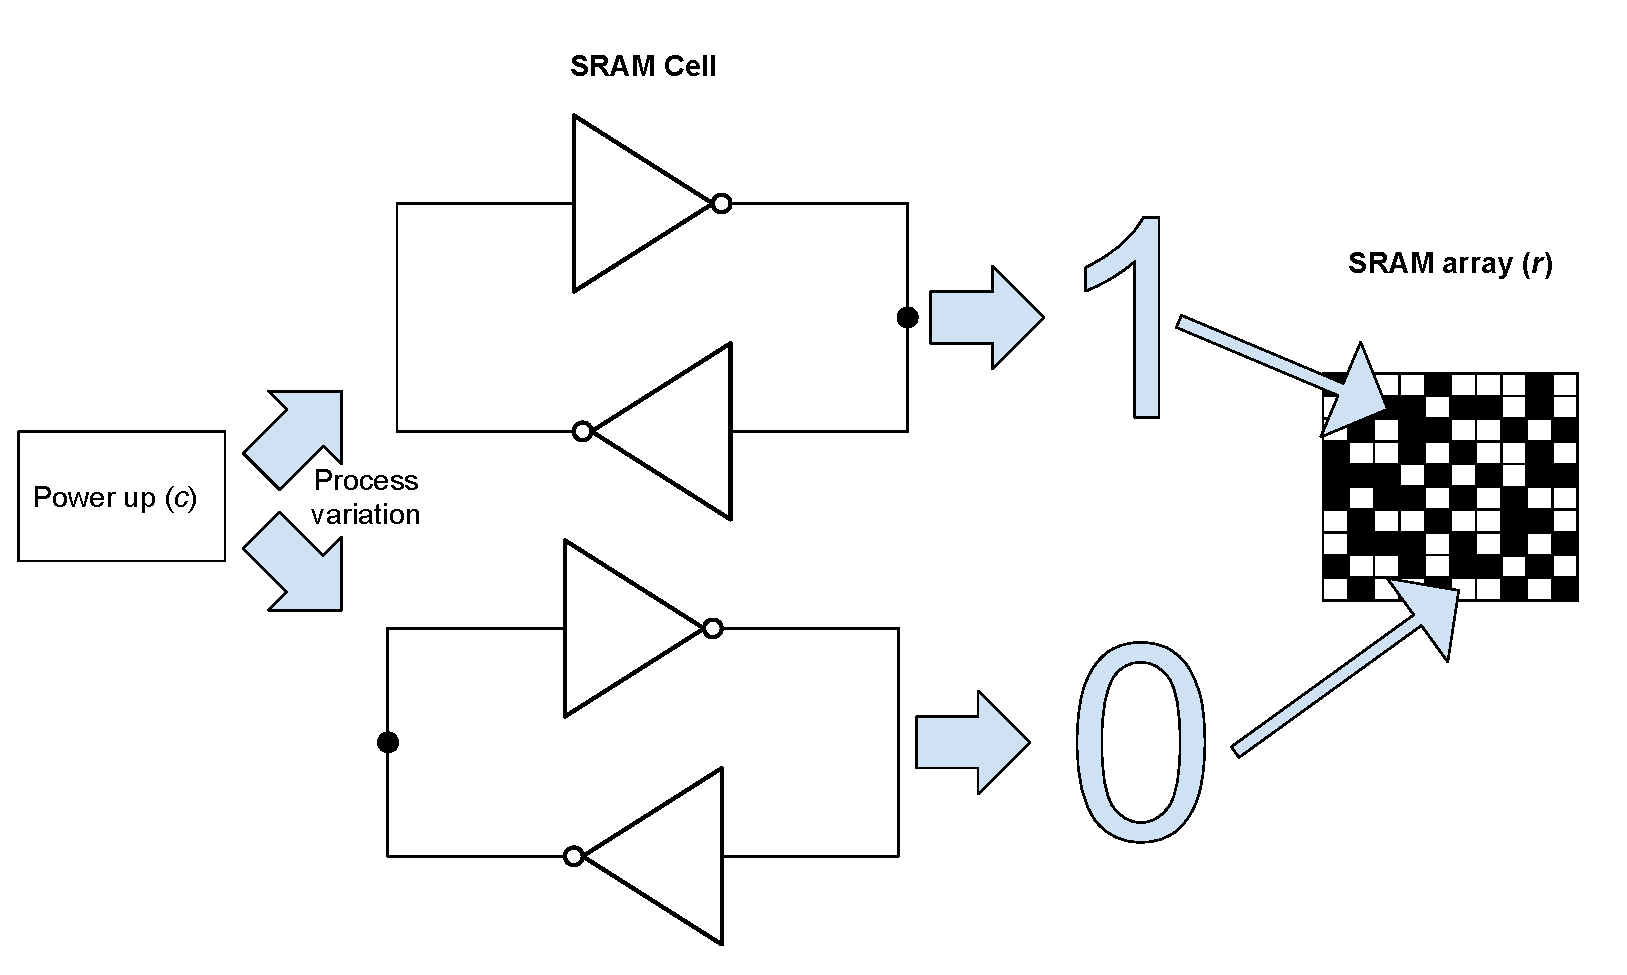
\includegraphics[width=14cm]{images/SRAM PUF implementation.pdf}
    \caption{Schematic of an SRAM PUF implementation.}
    \label{fig:SRAM_PUF}
\end{figure}

 SRAM PUFs are quite popular compared to other implementations \cite{Xiao2014,Zhang2020,Akhundov2019,Hofer2010} because they provide multiple advantages. SRAM memories are a ubiquitous device and a small fraction of a general purpose SRAM memory cells can also be used as PUF, in which case the PUF would come at almost no implementation cost. They have a low area and power consumption when compared to other PUFs and are easily scalable. Since SRAM memories have been a staple of electronic systems for a long time they are efficient, well characterized and understood. However, their main drawback is their limited reliability due to noisy responses. These PUFs will be the focus on this work so a more detailed description on the use of SRAM as PUFS is provided in the next chapter. Many studies have been published regarding the different aspects of SRAM PUFs and how to improve them due to the potential of the technology.

% SRAM cells are biased towards either ``1'' or ``0'' as explained before, but this bias can be strong or weak since it relies on the random distribution of process variation. Cells with a weak bias may sometimes power up in their non-preferred state due to noise or change in environmental conditions (bit flipping) and are considered unstable cells. Cells with a strong bias have a low probability of bit flipping and are considered stable cells. The distribution of the transistors' threshold voltage is assumed to be gaussian as in the mismatch models. In principle, this would make most values fall around the middle, so most cells should be unstable. Nonetheless, the bias does not have to be very strong to have a stable cell, so generally a majority of cells are considered stable \cite{Baturone2015,Bohm2013}. 






\section{Metrics}
\label{sec:Metrics}

Proper metrics are fundamental to evaluate the performance of PUFs and ensure their functionality in the applications shown in sec. \ref{sec:applications}. Their goal is to properly measure \textbf{Uniqueness}, \textbf{Reliability} and \textbf{Unpredictability} without redundant metrics. These characteristics have been explained qualitatively but they must be characterized quantitatively. There is a wide range of possibilities on which ones to use. A comprehensive list of metrics specifically created for PUFs can be found in \cite{Maiti2013}. PUF implementations usually provide a binary response either due to the physical property they measure or by applying some postprocessing after that measurement. Accordingly, the metrics used for PUFs are for binary strings of variable length. 


\subsection{Probability}
A fundamental concept in PUFs as a statistical process is the probability of occurrence of a “1” response, $p$. If the elements of a string of bits are random variables, their response corresponds to a binomial distribution \cite{Bohm2013}. This distribution is defined as: 
\begin{equation}
\label{eq:binomialpmf}
P(x=k)=
\left(\begin{array}{l}
n \\
k
\end{array}\right) p^{k}(1-p)^{n-k}\end{equation}

where $n$ is the number of bits in the bit string and $k$ the number of ``1'' responses. When the number of bits is sufficiently large, it can be approximated by a normal distribution which  significantly simplifies obtaining the probability. The probability density function for the normal distribution is: 

\begin{equation}f(x)=\frac{1}{\sigma \sqrt{2 \pi}} e^{-\frac{1}{2}\left(\frac{x-\mu}{\sigma}\right)^{2}}\end{equation}

where $\mu$ is the mean of the distribution and $\sigma$ is the standard deviation. The conversion from the binomial to the normal distribution is as follows:
\begin{equation}
\label{eq:conversion}
\begin{aligned}
\mu &=n p \\
\sigma^{2} &=n p q
\end{aligned}\end{equation}

Lastly, the mean of the normal distribution for $N$ binomial distributed data sets (DS) can be approximated as \cite{Bohm2013}:
\begin{equation}\mu_{a l l} \approx \frac{\# \text {of } 1 \text {'s in all  DS}}{n \cdot N}\end{equation}
And the probability of each cell is derived from here by using eq. \ref{eq:conversion}:

\begin{equation}
\label{eq:prob}
p=\frac{\mu_{a l l}}{n} \approx \frac{\# \text {of } 1 \text {'s in all  DS}}{N}
\end{equation} 

\subsection{Bit Error Rate}

The Bit Error Rate (BER) of a response is defined as the ratio between the number of false bits $e$ and the whole number of bits in a bit string $N$ \cite{Bohm2013}:
\begin{equation}
\label{eq:BER}
\text{BER}=\frac{e}{N}\cdot 100
\end{equation}

%  This metric is equivalent to the mean intra hamming distance \cite{Bohm2013}, commonly referred in the literature as fractional hamming distance.

It gives a clear measure of how error prone the PUF is. Accordingly, it helps to measure \textbf{Reliability}. The stability (number of correct bits) is complementary to the BER and usually only one of the two is given. To determine whether a bit is correct or false, first, there must be a string with the ideal or golden response for reference. This reference mask is calculated from the probability of each bit, if $p\geq 0.5$ the ideal value will be $1$ and if $p< 0.5$ the ideal value will be $0$. The mask can be determined directly from the evaluated dataset (intrinsically) or given as an input (extrinsically). The extrinsic reference is the golden response obtained under nominal conditions. It can be useful if, for example, the device is measured in varying conditions of voltage or temperature and a bit response switches from preferring 1s to 0s or vice versa. This would introduce a persistent error in the response when compared to the nominal conditions, but if the ideal string were determined intrinsically it would appear as if the cell was working properly. 

The BER can be obtained bit-wise ($N=1$) or response-wise ($N$ depends on the number of bits in the response). The second one gives a clear idea of the response quality and is generally the one used, although the first one can be useful for graphical representations (as in fig \ref{fig:BER}) or to obtain more detailed information about the behaviour of each bit. The ideal value for BER would be 0\% in either case.


\begin{figure}[H]
    \centering
    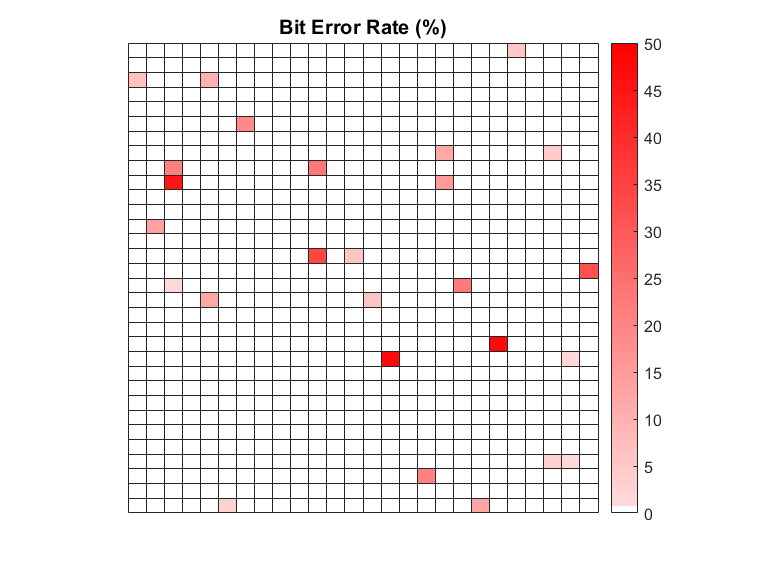
\includegraphics[width=10cm]{images/BERexample.png}
    \caption{Bit-wise representation of BER for a given dataset}
    \label{fig:BER}
\end{figure}
\subsection{Maximum intra hamming distance}

  The hamming distance between two strings is the number of different bits, i.e. the bits that need to be flipped for the two strings to be equal. The maximum intra hamming distance is the highest value among the $m$ hamming distances between each response to the same challenge and the golden response. This can be defined formally as:

\begin{equation}
\label{eq:maxihd}
\text{max}_\text{IntraHD}=\max _{i=1, \ldots, m}\left[\frac{H D\left(R_{ideal}, r_{i}\right)}{n}\right] \cdot 100\end{equation}

Where $n$ is the number of memory cells and $m$ the number of responses generated from the device. $R_{ideal}$ is the golden response and $r$ is one of $m$ responses. As in the BER the ideal response can be determined intrinsically or extrinsically. It is a measure of \textbf{Reliability} as well, but gives an idea of how bad the worst case scenario is instead of the general reliability of the device. Zero is the ideal value for this metric, since it means all responses to the same challenge are equal.

\subsection{Mean Inter Hamming distance}
\label{eq:interhd}
The mean inter hamming distance is calculated as the mean of the hamming distances between the golden responses of all chips. This is obtained through the following expression \cite{Maiti2013}:
\begin{equation}\text{mean}_\text{InterHD}=\frac{2}{k(k-1)} \sum_{i=1}^{k-1} \sum_{j=i+1}^{k} \frac{H D\left(R_{i}, R_{j}\right)}{n} \times 100 \%\end{equation}
Where $k$ is the number of chips. The $2/k(k-1)$ factor computes the mean. This metric gives a measure of the \textbf{Uniqueness} of the PUF. In the ideal case it is 50\%, meaning that the response of each chip is independent from each other. If uniqueness is low, knowing the response of one PUF would make predicting the response of other chips easier and security would be reduced.
\subsection{Hamming Weight}
Hamming weight simply measures the percentage of 1s in the $m$ responses to the same challenge:
\begin{equation}\text{HW}=\frac{1}{n\cdot m} \sum_{i=1}^{m} \sum_{l=1}^{n} b_{i,l} \cdot 100 \end{equation}
Where $b_{i,l}$ is the $l$-th binary bit of a $n$-bit response from a chip and $m$ is the number of responses. This metric provides an insight into the \textbf{Unpredictability} of the response, as a non uniform one where a certain state is favoured will make predicting the response easier. Ideally the result is 50\%, a balanced distribution of 1s and 0s. 

% \subsection{Minimum entropy}

% This metric is useful when evaluating the capabilities of a PUF as a random number generator instead of as an unique identifier. It summarizes the adequacy of $n$ memory cells to generate random numbers. Assuming that the $n$ memory cells have independent start-up values, the minimum entropy of the $n$-bit sequence (given as a percentage) is \cite{Baturone2015}:
% \begin{equation}H_{\min }=-\frac{1}{n} \sum_{i=1}^{n} \log _{2}\left(p_{i \max }\right) \cdot 100\end{equation}
% Where $p_{i \max }$ is the maximum probability of each cell to power-up to ‘0’ or ‘1’. It goes from 0\% for the absolutely reliable devices to 100\% where the probability of each cell is 0.5, an ideal random number generator. This means that it can be a measure of \textbf{Reliability} as well for unique identifiers, although BER covers that role better than minimum entropy since the result is a direct value for reliability. 








\section{Helper Data Algorithms} 
\label{sec:HDAs}
%Small introduction on the need for HDAs and their goal. 1 page.

For the sake of better understanding, so far the PUF has been considered ideal so that its response meets the specifications described in fig. \ref{fig:req}. However, due to environmental conditions (e.g. noise, polarization changes or temperature variations) and circuit aging, some response bits will not have a stable output and their value will change after repeating the same challenge, as shown in fig. \ref{fig:Unreliability}. This is known as the bit-flipping problem \cite{Baturone2015,Bhargava2012,Eiroa2012}. Bit-flipping is particularly problematic for silicon PUFs and, specifically, SRAM PUFs. Weak PUFs used as unique identifiers or to generate cryptographic keys must have perfect reliability, otherwise a legitimate PUF may be considered a fraudulent one. 


\begin{figure}[H]
    \centering
    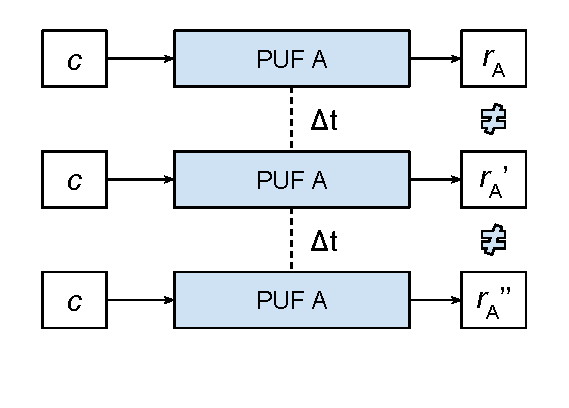
\includegraphics[width=8cm]{images/Unreliability.pdf}
    \caption{Illustration of the bit-flipping problem. The same PUF gives a different response to the same challenge at different points in time. }
    \label{fig:Unreliability}
\end{figure}

% Although HDAs can help to improve uniqueness, reliability and unpredictability, generally the focus is put on reliability.  
%  Sometimes, fuzzy extractors can be thought to be the same thing as HDAs, but there is a slight difference. Fuzzy extractors comprehend only a subset of all HDAs since they offer two guarantees: that the helper data does not reveal information about the key and that as long as the distance between the two readings is smaller than or equal to a constant $t$, the same key is extracted during the recreation step. These two guarantees are not present in HDAs.
In order to avoid this problem, HDAs are applied so that PUFs responses meet the required reliability specifications for key generation in any implementation \cite{Delvaux2015}. They transform noisy and non-uniform responses into reliable and uniformly distributed keys. To achieve this improvement, they require helper data.  These specifications depend on the implementation's demands (such as the mean time between two successive accesses) but a target used thorough the literature is a failure rate of less than $10^{-4}\ \%$ \cite{Bohm2013,Delvaux2015}. This means that the key has a chance of one in a million to be erroneous. The failure rate is also known as Key Error Rate (KER).  $10^{-4}\ \%$ is a reasonable target for a mean inter access time of one minute \cite{Alioto2019}. 

HDAs are applied in three consecutive steps: bit selection, error correction and entropy compression \cite{Delvaux2015}. Bit selection consists on using the most reliable bits out of the available ones. Error correction uses ECCs which lower the probability of failure by taking redundant bits. Finally, entropy compression uses a hash function to make the key uniform with perfect entropy and requires redundant bits as well. The need for these redundant bits means that the required PUF's response will be longer than the resulting key.

There is always a trade-off in terms of cost and improvement with each technique used. The goal when selecting a HDA is to meet the required specifications in the most efficient way possible. Bit selection, error correction and entropy compression are not mandatory, there are schemes that rely only on heavy error correction \cite{Bosch2008}, that do not require any error correction \cite{Liu2017} or that go without entropy compression \cite{Martinez-Rodriguez2018}.  

%It is important to keep in mind that enhancing the PUF's response can be achieved through design techniques to improve the output of the PUF itself, not just HDAs. 

The specific implementation of a HDA can take different forms \cite{Hiller2020}. Two common constructions are considered:  Code-offset, presented in \cite{Dodis2004} and applied for example in \cite{Maes2009,Bosch2008}, and fuzzy commitment presented in \cite{Juels1999} and applied in \cite{VanDerLeest2012soft,Kusters2017}. They are capable of reaching a similar level of reliability \cite{Yu2013} and employ the same type of ECCs. 

%Fuzzy commitment \cite{VanDerLeest2012},

In a code-offset construction two phases are required: Enrollment and Reconstruction. Enrollment, shown in fig. \ref{fig:HDA} (a), is performed only once in a secure environment and after manufacturing. In this phase, a codeword $c$ is generated with the error correction encoder by using a random secret $x$. The PUF response $r$ is employed to generate the key through a hash function. A XOR operation is performed on this response and the code word to generate the helper data $h$. In principle, helper data can be made public without compromising the security of the key, and may be stored in an internal NVM, an external memory, in a server, etc. Reconstruction, shown in fig. \ref{fig:HDA} (b), is in-the-field deployment, performed when the key is required. First, a XOR on the noisy PUF response $r'$ and the stored helper data results in a codeword $c'$. Then, if the number of errors does not exceed the tolerance of the code, the error correction decoder fixes the mistakes in $c'$ and returns $c$. Afterwards,  the original PUF response $r$ is recovered by performing a XOR on the codeword $c$ and the helper data. The original key is obtained after $r$ is hashed.  

%To reduce the impact of errors in this phase and since it is performed only once, taking the average of a number of CRPs can prove useful. \cite{Bohm2013}.     


\begin{figure}[H]
    \centering
    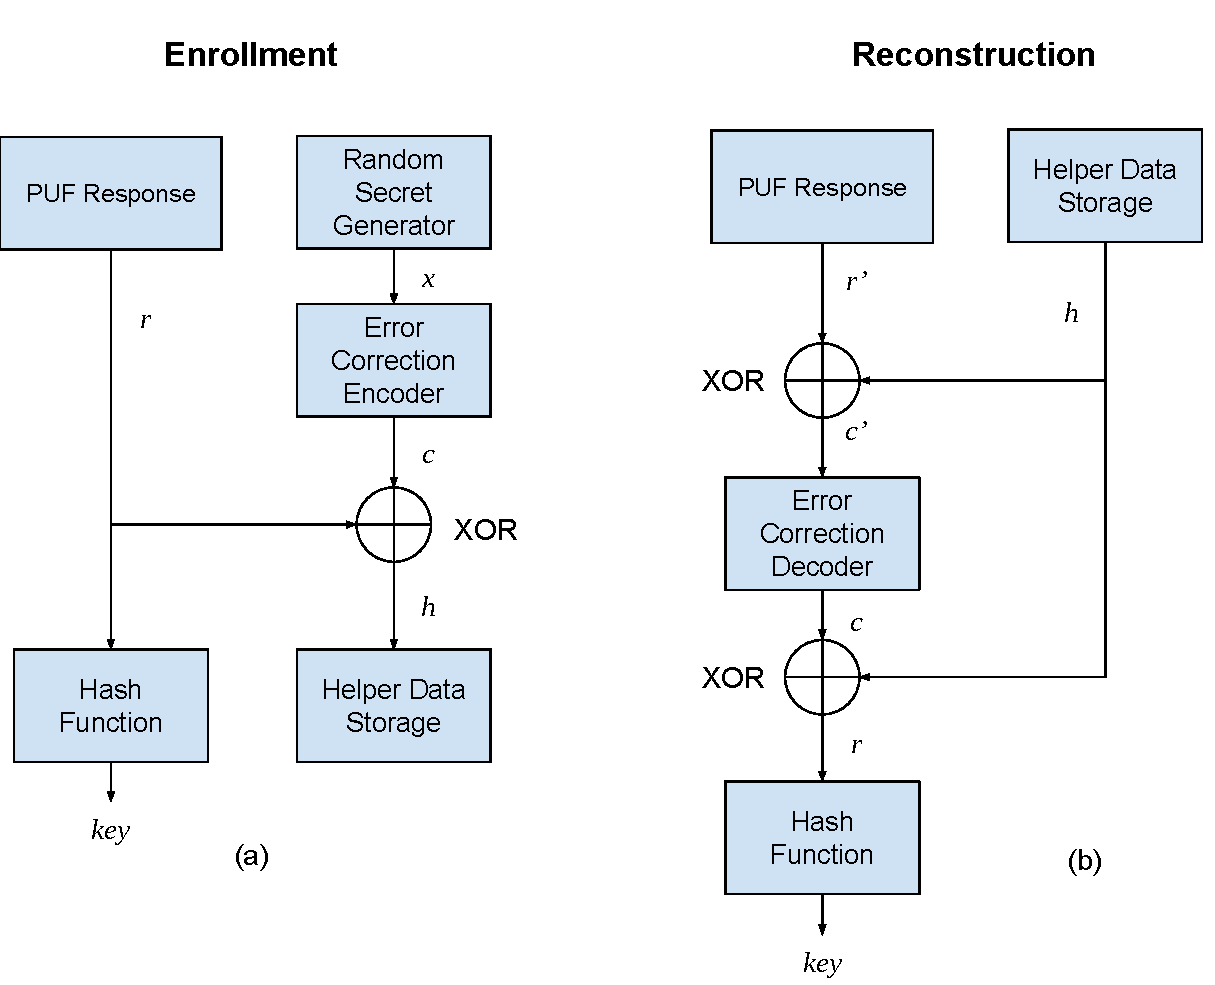
\includegraphics[width=12.5cm]{images/code offset.pdf}
    \caption{Helper data algorithm based on the code-offset construction. This algorithm has two phases: Enrollment (a) and Reconstruction (b).}
    \label{fig:HDA}
\end{figure}

In a fuzzy-commitment construction, the same two phases used in the code-offset construction are employed: Enrollment and Reconstruction. However, the approach in this construction is to obfuscate a randomly generated key or secret information through the PUF response instead of obtaining a key from the PUF response itself. In the Enrollment phase, shown in fig. \ref{fig:commitment}, $key$ is generated and then codified through the error correction encoder, obtaining $c$. Then, a XOR operation is performed on the codeword $c$ and the PUF response $r$ to obtain the helper data $h$, which is stored. During Reconstruction, $c'$ is obtained by performing a XOR on the noisy PUF response $r'$ and $h$. If the number of errors is low enough, $key$ is successfully recovered.

\begin{figure}[H]
    \centering
    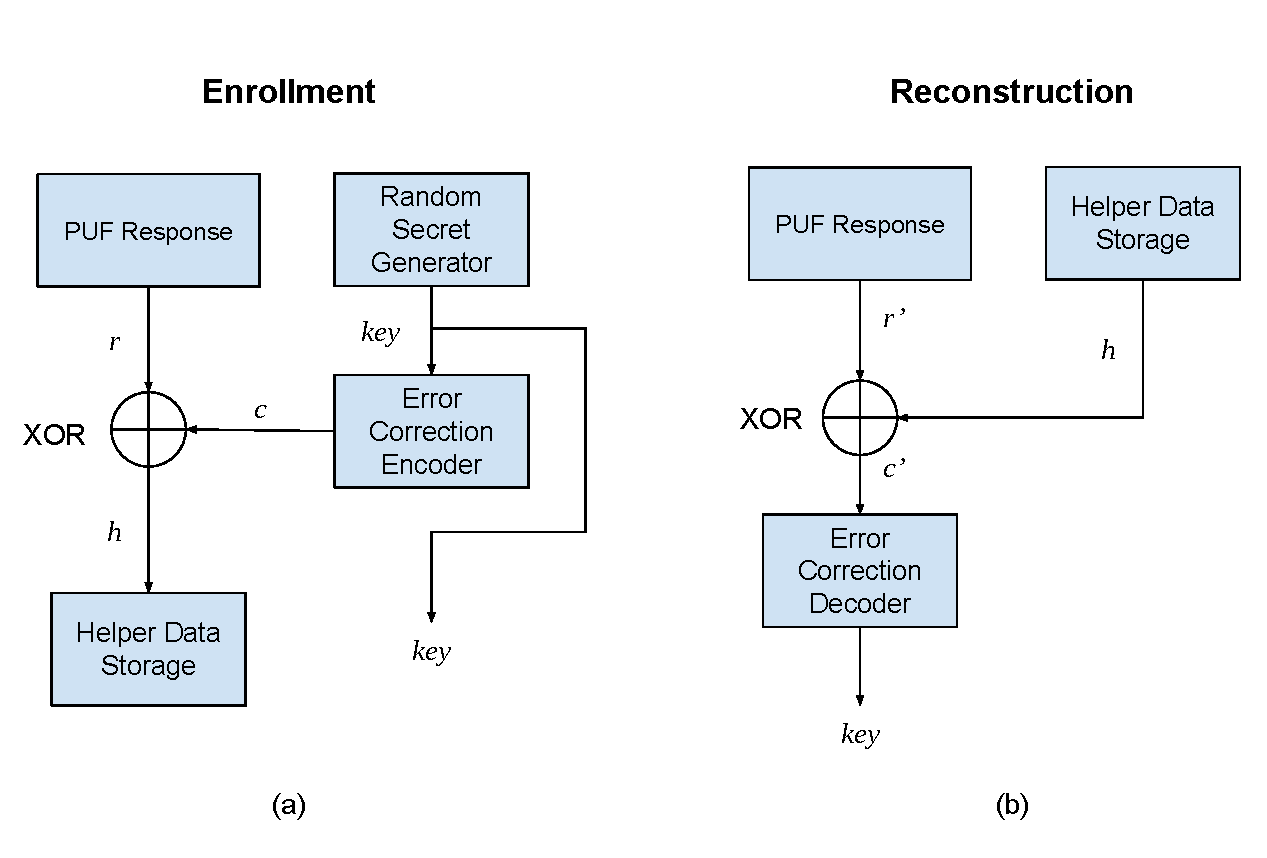
\includegraphics[width=13cm]{images/Fuzzy commitment.pdf}
    \caption{Helper data algorithm based on the fuzzy commitment construction. This algorithm has two phases: Enrollment (a) and Reconstruction (b).}
    \label{fig:commitment}
\end{figure}

Comparing both techniques, fuzzy commitment is simpler and easier to implement than code-offset. However, since it does not have a hash function, the helper data can leak information if the PUF response is non-uniform \cite{Dodis2004}.

In the next subsections bit selection techniques, ECCs and entropy compression are examined one by one.





\subsection{Bit selection}

% Selection based on Multiple evaluation, activation control, post silicon selection, directed accelerated aging (basically different methods found in the bibliography to reduce error before the error correction phase). Compilation of results from different approaches. 3-4 pages

Bit selection improves the output reliability by using as PUF only a subset of the available bits. Their goal is to reduce the requirements for the ECCs. In some cases this selection simply removes the unstable bits out of the pool of available bits and in others it tries to rank the bits according to their reliability so the best selection possible is used. 


Bit selection techniques vary according to the type of PUF employed. Since this work focuses on SRAM PUFs, only techniques applicable for SRAMs are considered. In these devices, the selection is done on the cells. For example, Multiple evaluation \cite{Baturone2015} is a widely used technique where all cells are powered up a number of times and those that do not always produce the same response are discarded. This is a straightforward technique but presents some drawbacks, as it requires many power ups and only discards unstable bits without making a classification of the stable ones. New bit selections techniques are sought, and some of them will be evaluated in chapter \ref{chap:4}, where a new selection technique is presented.


\subsection{ECCs}

\label{ss:ecc}

% Basic introduction and theory, Repetition, golay, BCH, Reed-Solomon... 3-4 pages


ECCs are a powerful and easy to scale tool to achieve any degree of reliability from a PUF response. They are well established since ECCs are of great importance in multiple fields such as computing, telecommunication or information theory to control errors in data over unreliable or noisy communication channels \cite{CastineiraMoreira2006}. ECCs are the most common way to implement forward error correction (FEC) \cite{CastineiraMoreira2006}. The central idea of FEC is to correct errors without requesting retransmission of the original information by introducing a known structure into a data sequence.

ECCs can be designed to correct bit-flips, bit-insertions and bit-deletion. The concern for PUFs is correcting bit-flips, so only ECCs geared towards this purpose are considered. In this work the PUF response is assumed to be a binary string, so only binary codes are evaluated.

The drawback of ECCs is their area and energy cost. These are around two orders of magnitude greater than the PUF itself \cite{Alioto2019} for common silicon PUF implementations and they increase linearly with the number of correcting bits \cite{Taneja2019}. On top of that, requiring redundant bits from the PUF comes at an expense that varies depending on the implementation. The rise in cost due to the increased hardware complexity provides a great incentive to reduce the unreliability of the response before applying the ECC.

%In most cases, the ECC is implemented with the worst case corner in mind. In \cite{Taneja2019} an architecture that adjusts the number of ECC bits required based on the actual instantaneous unstable bits is proposed. This saves up on energy requirements but not on area consumption. 

As explained before, ECCs require certain helper data obtained during the enrollment phase of the HDA. This helper data differs from one ECC to another, and many are available \cite{CastineiraMoreira2006}. To effectively choose one, an ECC can be evaluated through three criteria \cite{Xu2015}:

\begin{enumerate}
    \item \textbf{Error reduction:} Measured simply as the reduction in BER achievable through the ECC. 
    \item \textbf{Redundancy:} It is defined as the ratio of the number of bits required from the PUF to the length of the resulting key. As redundancy increases, so do the error correction capabilities, as well as the area and energy costs. Low redundancy is important if there is a constraint in the number of available bits in the PUF.
    \item \textbf{Complexity:} Some ECCs are harder to implement in hardware than others or require more computational time. This criteria is more complicated to evaluate as it is heavily dependent on the specific implementation, but it is nonetheless important to consider. If, for example, a specific code performs better in redundancy or error correction compared to another one but the cost of implementing it increases significantly, the benefits from better performance may not be worth.
    
\end{enumerate}

Each type of ECC offers advantages and disadvantages compared to the rest in terms of these criteria, and there is not a universally good choice. It is important to select the ECC that meets the requirements in the most efficient way possible, as the ideal choice may vary between implementations. Improving one of the criteria usually represents a trade-off with the others. 



 There are two categories of ECCs: block codes and convolutional codes \cite{CastineiraMoreira2006}. Block codes add fixed size block of bits to the initial message. A sequence of message bits is followed by a sequence of redundant bits, which forms the codeword. In convolutional codes, the redundant bits are spread along the codeword. The choice between block code and convolutional code depends on the application \cite{Johannesson2015}. Convolutional codes require a memory for encoding and decoding while block codes do not, which may be a limitation in certain implementations. Block codes are more established and easier to implement than convolutional codes \cite{CastineiraMoreira2006}, although the full potential of convolutional codes has not been reached yet \cite{Rachinger2015}.  Convolutional codes allow for on-the-fly decoding, which is very useful in continuous communications. Block codes require waiting for the entire codeword to start decoding. However, since PUF responses have a fixed length, they do not make use of this property, and convolutional codes are not as popular for PUF implementations since block codes seem like an easier and more obvious solution \cite{Maes2009}. For this reason, block codes will be examined in more detail. 
 
 

A block code $C$ obtains a codeword $c$ from a message $m$:
\begin{equation}
    c=C(m)
\end{equation} 

In this way, the block code maps the message to a unique codeword (encoding). The length of message $m$ is represented by $k$, while $n$ represents the length of codeword $c$. The redundancy can then be expressed as $R=k/n$. 

ECCs have a set of valid codewords in a certain space. The rest of possible codewords in that space are considered non-valid codewords. They are able to correct errors by changing non-valid codewords to their closest valid codeword and then decoding $c$ back to $m$. Accordingly, a key parameter in a block code is the distance $d$. It is defined as the minimum hamming distance between two valid code words. This distance provides a direct measure of the error correcting capabilities of the code: up to $d-1$ errors may be detected and up to $(d-1)/2$ corrected, rounded down.

%If the valid codewords are very different from each others, i.e. have a large $d$, many errors need to occur for an incorrect decoding.
The most important and commonly used ECCs are linear codes \cite{CastineiraMoreira2006}, which will be the ones considered here.
 A linear code is one where the linear combination of two valid codewords is a valid codeword. Linear binary block codes are represented with the notation $[n,k,d]$, which sets the parameters of a specific block code.
 


There are plenty of possibilities regarding block codes, but some of the most important ones and their strengths will be evaluated now in increasing order of complexity. After that, one convolutional code implementation for PUFs will be briefly examined. Lastly, different ECCs implemented in PUFs and their requirements will be compared. 

\subsubsection{Repetition Code}

% 
The repetition code $(R)$ is is the simplest code available. It obtains one bit of the key from $n$ bits of the PUF's response through majority vote, so $n$ must be odd and the redundancy is $n$. The distance in a repetition code is simply $n$. Some examples of PUF implementations that use this code can be found in \cite{Bohm2011,Maes2009,Martinez-Rodriguez2018}.
 
 To illustrate how this code work, a simple implementation using $R[3,1,3]$ for each bit of a 4-bit string will be examined in fig. \ref{fig:Repetition}. Initially the original message is encoded into four codewords by simply repeating each bit three times (fig. \ref{fig:Repetition} (a)). Two different examples are considered for decoding. In the first one, fig. \ref{fig:Repetition} (b), the codewords have three errors. However, they are spaced from each other and there is a majority of correct bits in each codeword. After doing a majority vote on each one, the original message is decoded. In the second one, fig. \ref{fig:Repetition} (c), the codewords have seven errors. In this case, two of them have a majority of errors and the resulting message is incorrect.
 
  \begin{figure}[H]
    \centering
    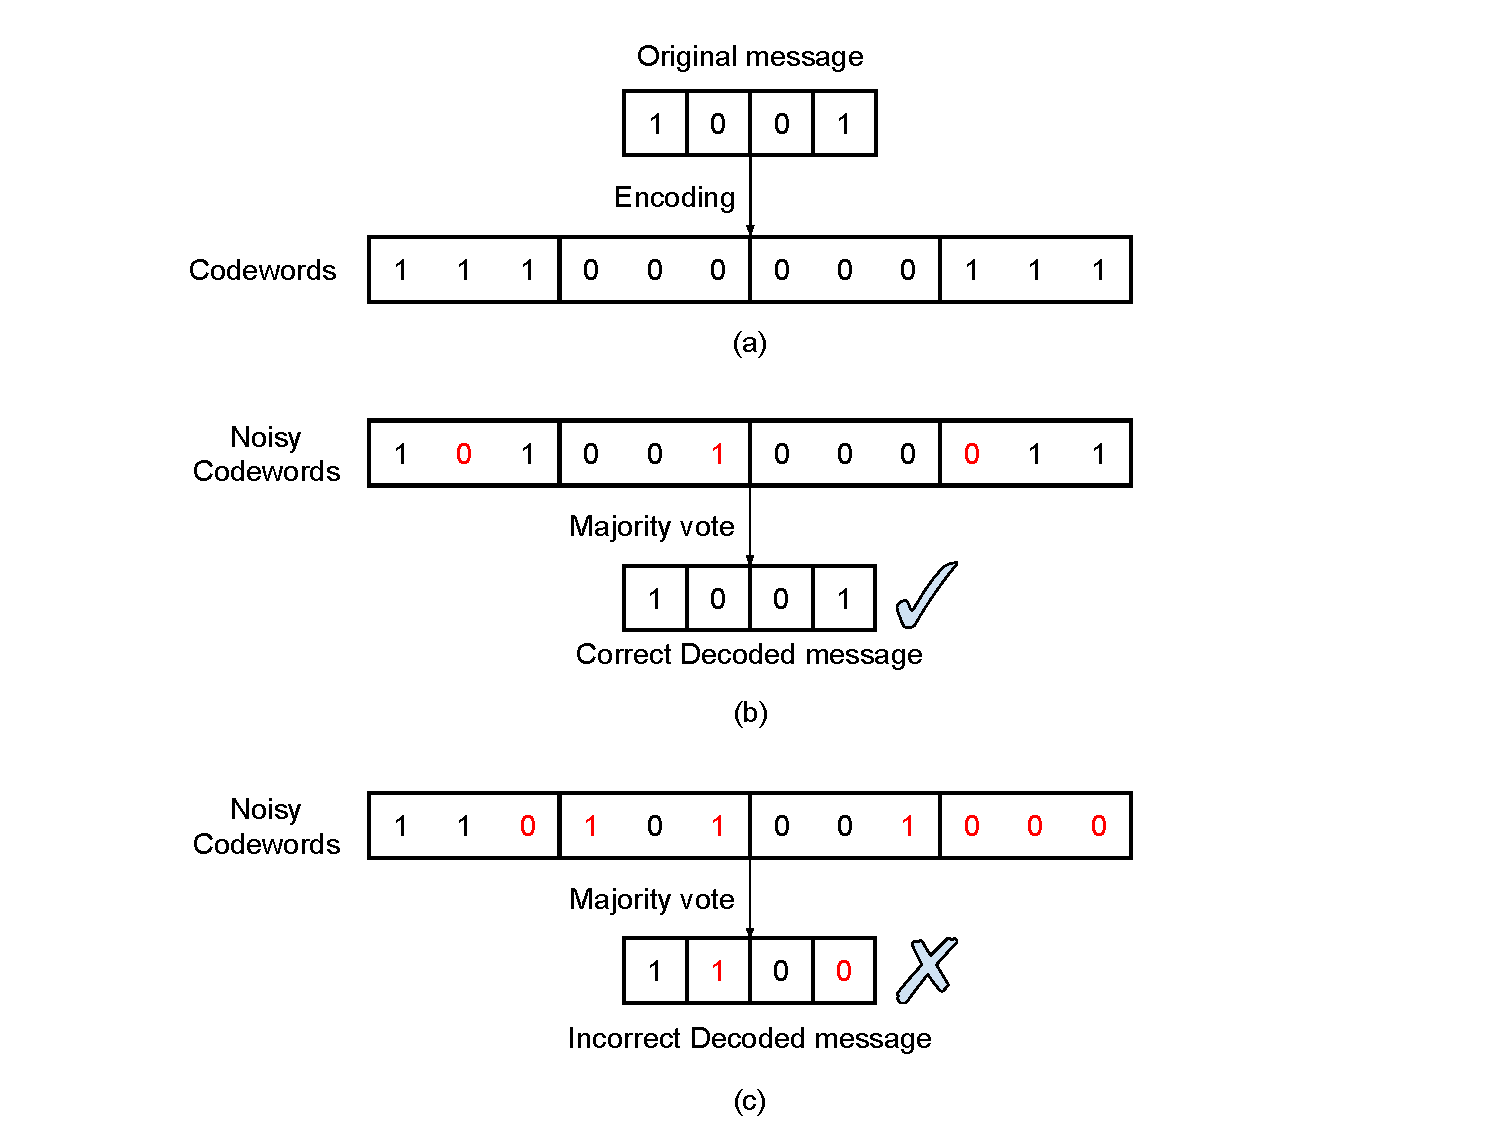
\includegraphics[width=13cm]{images/Repetition ECC.pdf}
    \caption{Repetition code $R[3,1,3]$ example for four bits. (a) shows the error correction encoding, (b) a successful decoding and (c) a failed decoding. }
    \label{fig:Repetition}
\end{figure}
 
In any case, if less than half of the $n$ bits of each codeword come with no error the original value will be recovered since the majority of bits will have the correct answer, otherwise it will fail. The error reduction capabilities of this code mostly depend on the initial BER. For a BER of $15-50 \%$, the $n$ required to meet specifications is prohibitively high, e.g. $n=33$ for a BER of $15\%$ \cite{Bohm2013}. However, if the BER is previously reduced, a repetition code with a small $n$ is pretty effective. 

This ECC has the highest redundancy possible, but its complexity is the lowest possible which makes it very easy to implement in any microcontroller. Repetition codes have entropy leakage issues, as pointed out by \cite{Delvaux2015,Koeberl2014}. These are specially significant for responses that are not perfectly uniform. 

\subsubsection{Hamming Code}

The hamming code was one of the earliest ECCs developed, in 1950 by Richard Hamming \cite{Hamming50}.  It employs parity checks through embedded parity bits to detect up to two-bit errors and correct up to one $(d=3)$. Parity checks consist in evaluating the parity of a set of bits and comparing it to a reference value, the parity bit. In binary, evaluating the parity of a set of bits is equivalent to performing a XOR operation. The most common hamming code is $Hamming[7,4,3]$, which has three parity bits $(p_1,p_2,p_3)$ and four message bits $(d_1,d_2,d_3,d_4)$. One way to graphically represent these bits is shown in fig. \ref{fig:HammingVenn}. 

\begin{figure}[H]
    \centering
    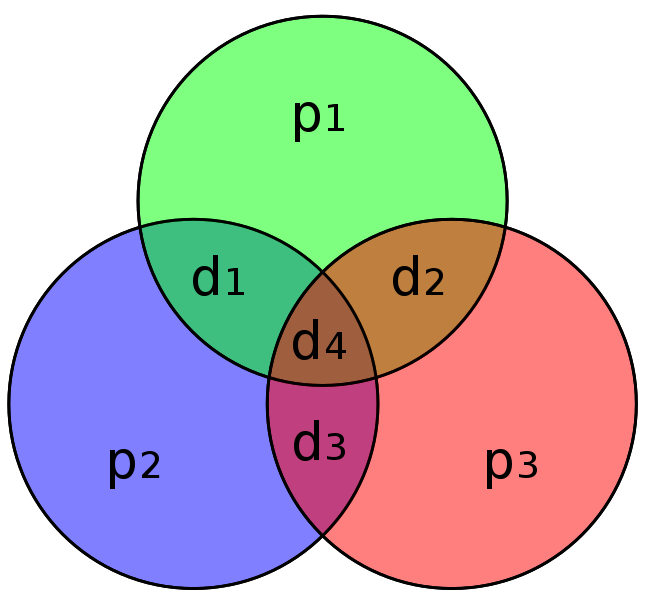
\includegraphics[width=5cm]{images/HammingVenn.png}
    \caption{Graphical depiction of the 4 data bits $d_1$ to $d_4$ and 3 parity bits $p_1$ to $p_3$ and which parity bits apply to which data bits \cite{Hammingwiki}.}
    \label{fig:HammingVenn}
\end{figure}



\begin{figure}[t]
    \centering
    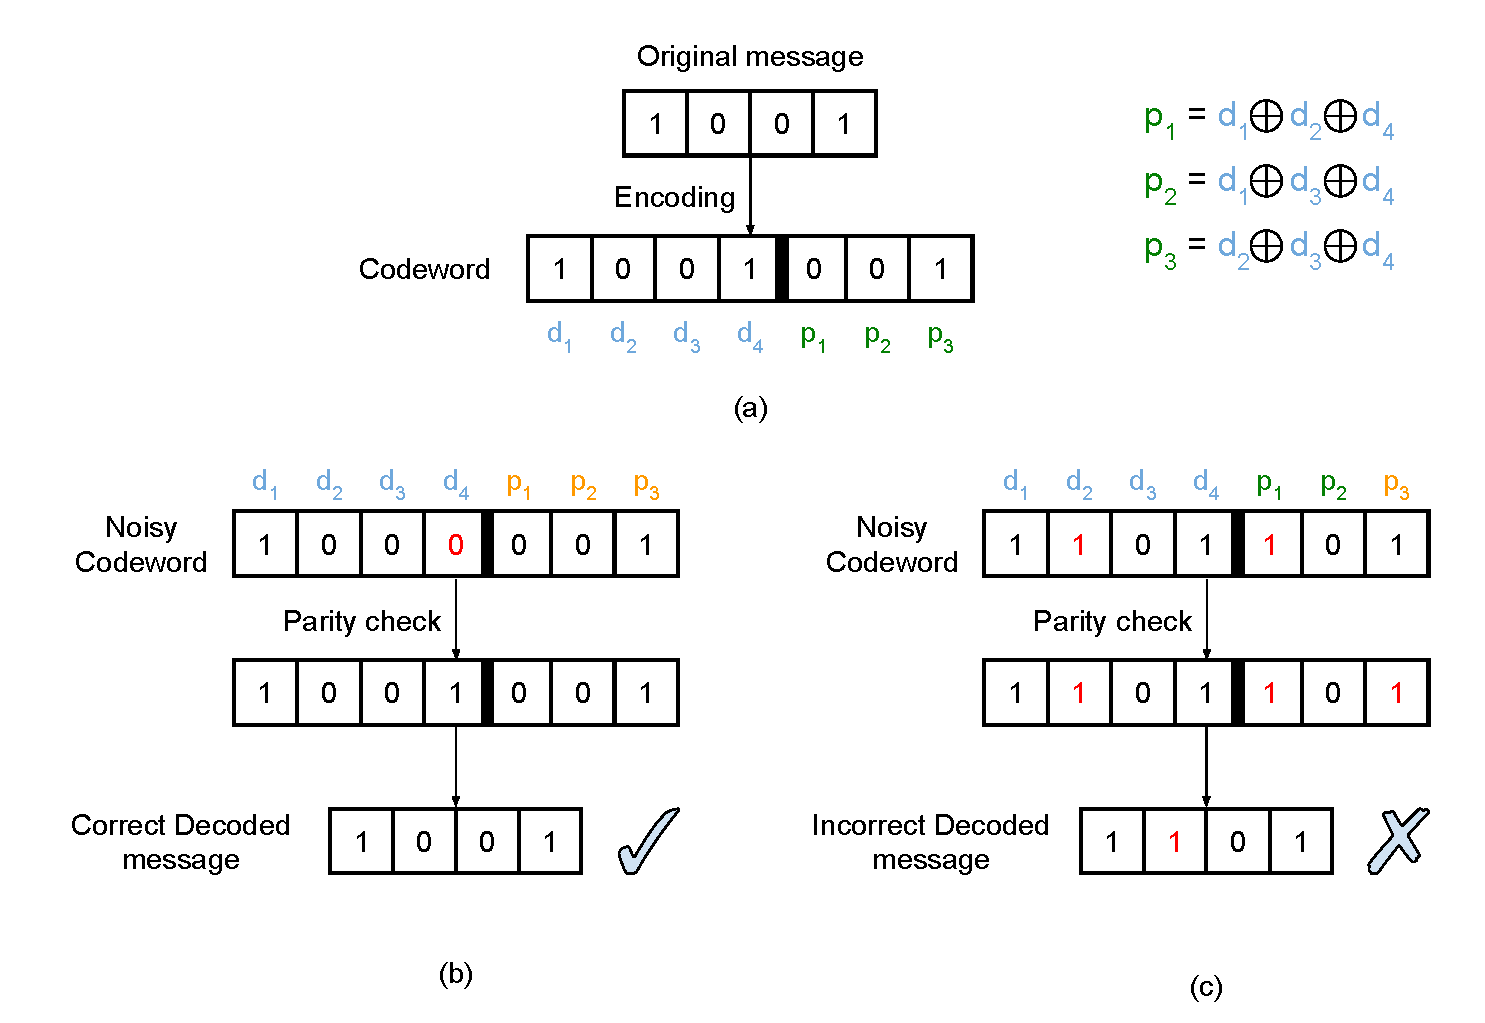
\includegraphics[width=12cm]{images/Hamming ECC.pdf}
    \caption{Hamming code $Hamming[7,4,3]$ example for four bits. (a) shows the error correction encoding, (b) a successful decoding and (c) a failed decoding. }
    \label{fig:HammingECC}
\end{figure}

Each parity bit checks three different combinations of three data bits. Error correction is performed by evaluating the parity bits, and the erroneous parity bits determine which bit has to be corrected. Suppose that there is one bit error. If one of the parity bits is incorrect, then the error is in that bit. If two are incorrect, either $d_1$, $d_2$ or $d_3$ (determined by the two parity bits) have a bit flip. If all three are incorrect, $d_4$ has the error. This is illustrated by a practical example in fig. \ref{fig:HammingECC}.

First, in fig. \ref{fig:HammingECC} (a), the original message is encoded by simply computing the parity bits and adding them to the message. Two different examples are considered for decoding. In the first one, in fig. \ref{fig:HammingECC} (b), the codeword has one error. Evaluating the parity bits reveals that $p_1$, $p_2$ and $p_3$ are wrong. If all three are incorrect, then $d_4$ has an error and gets corrected. The codeword is recovered and the message is correct. In the second one, in fig. \ref{fig:HammingECC} (c), the codeword has two errors. Evaluating the parity bits reveals that $p_3$ is wrong, so that bit gets corrected. Error correction failed because hamming codes can correct only one error, so the message is incorrect. 


Regarding their performance, redundancy in hamming codes is very good, as they use the minimum amount of parity bits for their length \cite{Huffman2003}. This ratio becomes even better as the length of the message $k$ increases.  Their complexity is high compared to repetition codes but low compared to more advanced codes as they only require a few XOR operations to perform parity checks. However, they have low error reduction capabilities, as they can only correct one error. Since most PUFs do not have low error rates, Hamming codes are not popular. 


\subsubsection{Reed-Muller code}

Reed-Muller (RM) codes are a big family of ECCs. They can be described in multiple ways. One clear explanation is provided in \cite{Abbe2020}. The code construction can be described as a greedy procedure, where the best set of codewords for each message $m$ with a length $k$ and a desired distance $d$ are sought. Consider building a binary linear code; it must contain the all-0 codeword. If one has to pick a second codeword, then the all-1 codeword is the best choice under any meaningful criteria. If now one has to keep these two codewords, the next best choice to maximize the code distance is to include the half-0 half-1 codeword and to continue building codewords sequentially. Once saturation is reached at relative distance $d$, it is less clear how to pick the next codeword, but one can simply take linear combinations of the previously picked codewords, and iterate this after each saturation. This procedure results in the valid set of $2^k$ RM codewords, so that each possible combination of $k$ bits has one codeword associated. 

% Another way to understand these codes comes from the fact that RM are considered polynomial codes. In polynomial codes, a string of $n$ bits can be identified with the polynomial:

% \begin{equation}
% a_{n-1} x^{n-1}+\cdots+a_{1} x+a_{0}
% \end{equation}

% For example, a bit string 11001 would be equivalent to $x^4+x^3+1$. In this way, the valid codewords are are those that are divisible by a certain fixed generator polynomial, which defines the code. RM codes with parameters $m$ and $d$ consist of all the evaluation vectors of polynomials with m variables and degree no larger than r \cite{Abbe2020}.

RM codes are often expressed as $RM(r,t)$, which corresponds to $RM\left[2^{t}, k, 2^{t-r}\right]$ in the standard notation. In this way, $n=2^t$ and $r$ represents the order of the code, an order by which the RM codes are classified. Reed-Solomon codes are one popular example of a high order RM code. However, for PUFs only RM codes of the first order are considered \cite{Bosch2008}, also known as augmented Hadamard codes. These codes are relatively easy to encode and decode by using majority-logic circuits, unlike higher order codes which require complex decoders. They are represented as $RM[2^{(k-1)},k,2^{(k-2)}]$, for a message $m$ of length $k$. These codes offer a middle ground between hamming and repetition in terms of redundancy and error correction capabilities, while being more complex than either of them. RM codes used in PUF implementations are found in \cite{Bosch2008,VanDerLeest2012soft,Hiller2015}. 



\subsubsection{BCH Code}

BCH stands for Bose–Chaudhuri–Hocquenghem, their inventors. They are cyclic codes, meaning that codewords generated through circular shifts of a valid codeword are a valid codeword. In a string of bits, a circular shift implies moving every bit to the left one position and the last bit to the beginning. Its capabilities are based on certain algebraic properties obtained from identifying each string of bits with a polynomial. However, an explanation of these properties is complex and beyond the scope of this work, so the focus will be on its practical features as ECCs. 

One of the main advantages of BCH codes is that they provide a wide variety of block lengths and corresponding code rates. All codewords will have a size $n=2^i-1$, where $i$ is an arbitrary integer greater than two. The corresponding $k$ and $d$ parameters have to be calculated for each possible $n$. For example, for $n=31$ the possible codes are $BCH[31,26,1]$, $BCH[31,21,2]$, $BCH[31,16,3]$, $BCH[31,11,1]$ and $BCH[31,6,7]$. 

BCH codes use similar decoding algorithms as RM \cite{Guruswami2010} so their complexity is similar. They offer better redundancy, close to Hamming codes, and the error correction capability depends on the parameters chosen. All of these facts make BCH codes a popular choice for PUFs \cite{Delvaux2015,Bosch2008,Maes2012pufky}. 

\subsubsection{Viterbi}

In contrast with the proposed block codes so far, the Viterbi algorithm is a decoding algorithm for convolutional codes. In convolutional codes, the output code bits are continuously determined by logic operations (generally shifts and XORs) on the present input bit in a stream and a small number of previous bits, so a memory is required for encoding and decoding. Viterbi algorithms find the most likely sequence of hidden states (the message) that result in a sequence of observed events (the measured code bits). Error correction is based on the fact that a low number of erroneous bits are not influential enough to change the most likely sequence of hidden states.

PUFs implementations of convolutional codes with Viterbi algorithms are found in \cite{Hiller2013,Hiller2014}. These show promising results, outperforming block-code implementations in error correction capabilities and redundancy. Their main drawbacks are higher complexity and response times \cite{Hiller2013}. 

\subsubsection{Comparison of ECCs in PUFs}

In essence, there are many possibilities regarding ECCs. There has been a lot of effort by the scientific community to try and find progressively better codes, due to how promising PUFs are. A combination of ECCs in two or more stages (concatenated code) can make use of the strengths of two different codes \cite{Bohm2013,Bosch2008} and are quite popular. For two codes, $C_1$ and $C_2$, the message is codified by applying first $C_2$ and then $C_1$. The message is later decoded by applying first $C_1$ and then $C_2$.

Table \ref{tab:ECCs} shows different ECC implementations found in the literature. All of these extract a 128-bit key from a PUF response that is presumed to have an average BER of 15 \%, a very safe estimate even under the worst corners of reliability \cite{Maes2009}.   A fair comparison in terms of how costly the hardware implementation will be is hard to make as it is heavily dependant on the specific technology used, so only the required PUF size and final KER are shown. However, it is an important factor to keep in mind. It is important as well to distinguish between soft- and hard-decision decoding \cite{Hiller2013}. For hard decision decoding, all codeword bits have the same weight and contribute equally to decoding. Meanwhile, soft decision decoding uses reliability information about each bit to increase efficiency, increasing the error correction capabilities at the cost of higher complexity. Soft decision decoding is employed in \cite{Maes2009,VanDerLeest2012soft}.

\begin{table}[H]
  \centering
  \caption{Comparison of different ECC approaches with aimed KER 1 E-4 \% showing required PUF bits and redundancy for a key length of 128 bits and a presumed BER of 15\%. }
  \resizebox{\linewidth}{!}{%
    \small
    \begin{tabular}{|c|c|c|c|c|c|}
    \hline
    Reference   & $C_1$   & $C_2$ & PUF bits & Redundancy & KER (\%)  \bigstrut\\
    \hline
    \cite{Bosch2008}   & $R[33,1,33]$ & - & 5643 & 33 & 1 E-4 \bigstrut\\
    \hline
    \cite{Bosch2008}   & $BCH[1023,46,439]$ & - & 4092 & 23.92 &1.85 E-6 \bigstrut\\
    \hline
    \cite{Bosch2008}   & $R[3,1,3]$ & $BCH[127,7,31]$ & 2286 & 13.37  & 8.48 E-4 \bigstrut\\
    \hline
    \cite{Bosch2008}   & $R[7,1,7]$ & $RM[16,5,8]$ & 3920 & 22.92 & 3.47 E-4 \bigstrut\\
    \hline
    
    \cite{Maes2009}   & $R[3,1,3]$ & $RM[64,22,16]$ & 1536 & 8.98 & 1 E-6 \bigstrut\\ %KER from Koeberl
    \hline
    \cite{VanDerLeest2012soft}   & $R[14,1,14]$ & $RM[8,4,4]$ & 4816 & 28.16 & 3.3 E-5 \bigstrut\\ %KER from Koeberl
    \hline
    \cite{Hiller2016}   & Viterbi & - & 974 & 7.61 & 7.94 E-5 \bigstrut\\
    \hline
\end{tabular}%
}
  \label{tab:ECCs}%
\end{table}%

It is clear that a large amount of PUF bits are required to obtain a 128-bit key, around five to fifty times the actual key size. This helps illustrate how costly ECCs are, and why there is such a motivation to preemptively reduce the PUF's BER by any means possible. 


\subsection{Entropy compression}

The entropy of the response is non-maximum due to intrinsic correlation and bias introduced in the PUF, as well as leakage from the HDA \cite{Delvaux2015}. By using this information, an attacker can reduce the search space required to obtain the secret key. A hash function solves this problem, as first proposed in \cite{Gassend2002}. This step is also known as privacy amplification.  Hash functions require more input than output bits and work by compressing the entropy of the input into a shorter output. In this way, the total amount of entropy remains constant but the entropy per bit increases. The hash function breaks the link between responses and physical details of the PUF as well, adding one more layer of security and making model-building attacks much more difficult. Entropy compression further increases the amount of bits required out of the ECC and, accordingly, the amount of bits required out of the PUF. 

In \cite{Guajarado_og,Bhargava2014}, the entropy per bit of an SRAM PUF is estimated to be at around 0.75. To achieve a perfect entropy per bit of 1, $N/0.75$ bits are required \cite{Guajarado_og} where $N$ is the length of the key. This would be 171 bits for a 128-bit key or 342 bits for a 256-bit key. There are a variety of hash functions available with their advantages and drawbacks. A popular implementation is the SPONGENT lightweight hash function \cite{Hiller2014, Maes2012}. An implementation of SHA-256 that is lightweight as well is found in \cite{VanDerLeest2012}. The more bulky universal Toeplitz hash is used in \cite{Maes2009}.